\documentclass{article}

\usepackage[margin=1in]{geometry}
\usepackage{amsmath, amssymb}
\usepackage{graphicx}
\usepackage{tikz}
\usetikzlibrary{fit}
\usepackage{circuitikz}
\usepackage{amsmath,blkarray,booktabs, bigstrut}
\usepackage[normalem]{ulem}
\usepackage{xcolor}
\usepackage{centernot}
\usepackage{multirow}
\usepackage{hhline}
\usepackage{etoolbox}
\AtBeginEnvironment{align}{\setcounter{equation}{0}}
\usepackage{fancyhdr}
\pagestyle{fancy}

\usepackage{hyperref}
\hypersetup{
    colorlinks=true,
    linkcolor=black,
    filecolor=magenta,      
    urlcolor=cyan,
}

\title{Discrete Math for Computer Science}
\author{Peter Schaefer}
\date{Freshman Fall}

\begin{document}

\maketitle

\tableofcontents

\newpage

\section{Logic}
\subsection{Propositions and Logical Operations}

\textbf{Proposition}: a statement that is either \underline{true} or \underline{false}.


Some examples include "It is raining today" and "$3 \cdot 8 = 20 $".


However, not all statements are propositions, such as "open the door"

\begin{center}
  \begin{tabular}{c|c|c}
    \textbf{Name} & \textbf{Symbol} & \textbf{alternate name} \\
    \hline
    NOT           & $\lnot$         & negation                \\
    AND           & $\land$         & conjunction             \\
    OR            & $\lor$          & disjunction             \\
    XOR           & $\oplus$        & exclusive or            \\
  \end{tabular}
  \qquad
  \begin{tabular}{c|c|c|c|c|c}
    \textbf{$p$} & \textbf{$q$} & \textbf{$\lnot p$} & \textbf{$p \land q$} & \textbf{$p \lor q$} & \textbf{$p \oplus q$} \\
    \hline
    T            & T            & F                  & T                    & T                   & F                     \\
    T            & F            & F                  & F                    & T                   & T                     \\
    F            & T            & T                  & F                    & T                   & T                     \\
    F            & F            & T                  & F                    & F                   & F                     \\
  \end{tabular}
\end{center}

XOR is very useful for encryption and binary arithmetic.

\subsection{Evaluating Compound Propositions}

\begin{align*}
  p & : \text{The weather is bad.}    & p \land q            & : \text{The weather is bad \textit{and} the trip is cancelled}                            \\
  q & : \text{The trip is cancelled.} & p \lor q             & : \text{The weather is bad \textit{or} the trip is cancelled}                             \\
  r & : \text{The trip is delayed.}   & p \land (q \oplus r) & : \text{The weather is bad \textit{and} either the trip is cancelled \textit{or} delayed} \\
\end{align*}

\textbf{Order of Evaluation} $\lnot$, then $\land$, then $\lor$, but parenthesis always help for clarity.

\begin{center}
  Example Truth Table:
  \qquad
  \begin{tabular}{c|c|c|c|c}
    $p$ & $q$ & $p \land q$ & $\lnot q$ & $(p \land q) \oplus \lnot q$ \\
    \hline
    T   & T   & T           & F         & T                            \\
    T   & F   & F           & T         & T                            \\
    F   & T   & F           & F         & F                            \\
    F   & F   & F           & T         & T                            \\
  \end{tabular}
\end{center}

\subsection{Conditional Statements}

\begin{center}
  $p \implies q$ \ where $p$ is the \underline{hypothesis} and $q$ is the \underline{conclusion}
\end{center}

\begin{center}
  \begin{tabular}{c|c}
    Format                     & Terminology    \\
    \hline
    $p \implies q$             & given          \\
    $\lnot q \implies \lnot p$ & contrapositive \\
    $q \implies p$             & converse       \\
    $\lnot p \implies \lnot q$ & inverse        \\
  \end{tabular}
  \qquad
  \begin{tabular}{ccccc}
    given   & $p \implies q$             & $\equiv$ & $\lnot q \implies \lnot p$ & contrapositive \\
    inverse & $\lnot p \implies \lnot q$ & $\equiv$ & $q \implies p$             & converse
  \end{tabular}
\end{center}

\begin{center}
  \begin{tabular}{c|c|c}
    $p$ & $q$ & $p \implies q$ \\
    \hline
    T   & T   & T              \\
    T   & F   & F              \\
    F   & T   & T              \\
    F   & F   & T              \\
  \end{tabular}
  \quad
  \begin{tabular}{c}
    $p$ is a \underline{sufficient} condition for $q$ \\
    $q$ is a \underline{necessary} condition for $p$
  \end{tabular}
  \quad
  \begin{tabular}{c|c}
    Phrase                 & Logic          \\
    \hline
    $q$ if $p$             & $p \implies q$ \\
    $q$ only if $p$        & $q \implies p$ \\
    $q$ if and only if $p$ & $p \iff q$
  \end{tabular}
\end{center}

\begin{center}
  \textbf{Order of Operations}: $p \land q \implies r \equiv (p \land q) \implies r$
\end{center}

\subsection{Logical Equivalence}

\begin{center}
  \textbf{Tautology}: a proposition that is always \underline{true}
  \qquad
  \textbf{Contradiction}: a proposition that is always \underline{false}
\end{center}

\textbf{Logically equivalent}: same truth value regardless of the truth values of their individual propositions

\textbf{DeMorgan's Laws}:
\qquad
\begin{tabular}{c}
  $\lnot (p \lor q) \equiv \lnot p \land \lnot q$ \\
  $\lnot (p \land q) \equiv \lnot p \lor \lnot q$
\end{tabular}

\begin{center}
  \begin{tabular}{c}
    Verbally,                                                                                   \\
    It is not true that the patient has migraines \textit{or} high blood pressure $\equiv$      \\
    $\equiv$ The patient does not have migraines \textit{and} does not have high blood pressure \\
    \hline
    It is not true that the patient has migraines \textit{and} high blood pressure $\equiv$     \\
    $\equiv$ The patient does not have migraines \textit{or} does not have high blood pressure  \\
  \end{tabular}
\end{center}

\subsection{Laws of Propositional Logic}

\begin{center}
  You can use \textbf{substitution} on logically equivalent propositions.
\end{center}

\begin{center}
  \begin{tabular}{r|c|c}
    \textbf{Law Name} & $\lor$ or                                               & $\land$ and                                              \\
    \hline
    Idempotent        & $p \lor p \equiv p$                                     & $p \land p \equiv p$                                     \\
    Associative       & $(p \lor q) \lor r \equiv p \lor (q \lor r)$            & $(p \land q) \land r \equiv p \land (q \land r)$         \\
    Commutative       & $p \lor q \equiv q \lor p$                              & $p \land q \equiv q \land p$                             \\
    Distributive      & $p \lor (q \land r) \equiv (p \lor q) \land (p \lor r)$ & $p \land (q \lor r) \equiv (p \land q) \lor (p \land r)$ \\
    Identity          & $p \lor $ F $\equiv p$                                  & $p \land $ T $\equiv p$                                  \\
    Domination        & $p \lor $ T $\equiv $ T                                 & $p \land $ F $\equiv $ F                                 \\
    Double Negation   & $\lnot \lnot p \equiv p$                                                                                           \\
    Complement        & $p \lor \lnot p \equiv$ T                               & $p \land \lnot p \equiv$ F                               \\
    DeMorgan          & $\lnot (p \lor q) \equiv \lnot p \land \lnot q$         & $\lnot (p \land q) \equiv \lnot p \lor \lnot q$          \\
    Absorption        & $p \lor (p \land q) \equiv p$                           & $p \land (p \lor q) \equiv p$                            \\
    Conditional       & $p \implies q \equiv \lnot p \lor q$                    & $p \iff q \equiv (p \implies q) \land (q \implies p)$
  \end{tabular}
\end{center}

\subsection{Predicates and Quantifiers}

\textbf{Predicate}: a logical statement where truth value is a \underline{function} of a variable.

\begin{center}
  P($x$): $x$ is an even number. \qquad P(5): false \qquad P(2): true
\end{center}

\noindent \textbf{Domain}: the set of all possible values for a variable in a predicate.

\begin{center}
  Ex. $ \mathbb{Z}^+ $ is the set of all positive integers.

  *If domain is not clear from context, it should be given as part of the definition of the predicate.
\end{center}

\noindent \textbf{Quantifier}: converts a predicate to a proposition.
\qquad
\begin{tabular}{c|c|c}
  Quantifier  & Symbol     & Meaning        \\
  \hline
  Universal   & $\forall$ & "for all"      \\
  Existential & $\exists$  & "there exists" \\
\end{tabular}

\begin{center}
  $\exists~ x (x+1 < x)$ is false.
\end{center}

\noindent \textbf{Counter Example}: universally quantified statement where an element in the domain
for which the predicate is false. Useful to prove a $\forall~$ statement false.

\subsection{Quantified Statements}

Consider the two following two predicates:
\begin{align*}
  P(x) & : x \text{ is prime, } x \in \mathbb{Z}^+ \\
  O(x) & : x \text{ is odd}
\end{align*}

\begin{center}
  Proposition made of predicates: \qquad $\exists~ x (\text{P}(x) \land \lnot \text{O}(x))$ \\
  Verbally: there exists a positive integer that is prime but is \underline{not} odd.
\end{center}

\noindent \textbf{Free Variable}: a variable that is free to be any value in the domain.

\noindent \textbf{Bound Variable}: a variable that is bound to a quantifier.

\begin{center}
  \begin{tabular}{rl}
    $\text{P}(x)$: & $x \text{ came to the party}$ \\
    $\text{S}(x)$: & $x \text{ was sick}$          \\
  \end{tabular}
  \qquad
  \begin{tabular}{c}
    $\text{P}(x) \overset{?}{\equiv} \lnot \text{S}(x)$ \\
    $\text{P}(x) \centernot{\equiv} \lnot \text{S}(x)$
  \end{tabular}
  \qquad
  \begin{tabular}{c|ccc}
         & P$(x)$ & S$(x)$ & $\lnot$S$(x)$ \\
    \hline
    Joe  & T      & F      & T             \\
    Theo & F      & T      & F             \\
    Gert & T      & F      & T             \\
    Sam  & F      & F      & T
  \end{tabular}
\end{center}

\subsection{DeMorgan's law for Quantified Statements}


Consider the predicate: F$(x):$ "$x$ can fly", where $x$ is a bird.
According to the DeMorgan Identity for Quantified Statements,

\begin{align*}
  \lnot \forall~ x \text{F}(x)    & \equiv \exists~ x \lnot \text{F}(x)                 \\
  \text{"not every bird can fly} & \equiv \text{"there exists a bird that cannot fly}
\end{align*}

Example using DeMorgan Identities:
\begin{align*}
  \lnot \exists~ x (\text{P}(x) \implies \lnot \text{Q}(x)) & \equiv \forall~ x \lnot (\text{P}(x) \implies \lnot \text{Q}(x))          \\
                                                           & \equiv \forall~ x (\lnot \lnot \text{P}(x) \land \lnot \lnot \text{Q}(x)) \\
                                                           & \equiv \forall~ x (\text{P}(x) \land \text{Q}(x))
\end{align*}

\subsection{Nested Quantifiers}

A logical expression with more than one quantifier that binds different variables in the same predicate
is said to have \textbf{Nested Quantifiers}.

\begin{center}
  \begin{tabular}{c|c}
    Logic                                    & Variable Boundedness     \\
    \hline
    $\forall~ x \exists~ y \text{ P}(x, y)$    & $x$, $y$ bound           \\
    $\forall~ x \text{ P}(x, y)$              & $x$ bound, $y$ free      \\
    $\exists~ x \exists~ y \text{ T}(x, y, z)$ & $x$, $y$ bound, $z$ free \\
  \end{tabular}
  \quad
  \begin{tabular}{c|c}
    Logic                                 & Meaning                              \\
    \hline
    $\forall~ x \forall~ y \text{ M}(x, y)$ & "everyone sent an email to everyone" \\
    $\forall~ x \exists~ y \text{ M}(x, y)$ & "everyone sent an email to someone"  \\
    $\exists~ x \forall~ y \text{ M}(x, y)$ & "someone sent an email to everyone"  \\
    $\exists~ x \exists~ y \text{ M}(x, y)$ & "someone sent an email to someone"   \\
  \end{tabular}
\end{center}

\noindent There is a two-player game analogy for how quantifiers work:

\begin{center}
  \begin{tabular}{c|c|c}
    Player                       & Action                                          & Goal                                       \\
    \hline
    Existential Player $\exists~$ & selects value for existentially-bound variables & tries to make expression \underline{true}  \\
    Universal Player $\forall~$   & selects value for universally-bound variables   & tries to make expression \underline{false}
  \end{tabular}
\end{center}

\noindent Consider the predicate L$(x,y):$ "$x$ likes $y$".
\begin{align*}
  \exists~ x \forall~ y \text{L}(x, y)       & \text{ means "there is a student who likes everyone in the school".}  \\
  \lnot \exists~ x \forall~ y \text{L}(x, y) & \text{ means "there is no student who likes everyone in the school".}
\end{align*}
After applying DeMorgan's Laws,
\begin{align*}
  \forall~ x \exists~ y \lnot \text{L}(x, y) & \text{ means "there is no student who likes everyone in the school".}
\end{align*}

\subsection{More Nested Quantifiers}

M$(x, y):$ "x sent an email to y". Consider $\forall~ x \forall~ y$ M $(x, y)$.
It means that "email sent an email to everyone including themselves".
Using $( x \not = y \implies \text{ M}(x, y))$ can fix this quirk.
\begin{align*}
  \forall~ x \forall~ y (x \not = y \implies \text{ M}(x, y))
  \text{ means "everyone sent an email to everyone else}
\end{align*}

\subsubsection*{Expressing Uniqueness in Quantified Statements}

Consider L($x$): $x$ was late to the meeting. If someone was late to the meeting,
how could you express that that someone was the only person late to the meeting?
You want to express that there is someone where everyone else was not late, which
can be done with
\begin{align*}
  \exists~ x (\text{L}(x) \land \forall~ y (x \not = y \implies \lnot \text{L}(y)))
\end{align*}

\subsubsection*{Moving Quantifiers in Logical Statements}

Consider M($x, y$): "$x$ is married to $y$" and A($x$): "$x$ is an adult".
One way of expressing "For every person $x$, if $x$ is an adult, then
there is a person $y$ to whom $x$ is married to" is by this statement:
\begin{align*}
  \forall~ x (\text{ A}(x) \implies \exists~ \text{ M}(x, y))
\end{align*}
Since $y$ does not appear in A($x$), "$\exists~ y$" can be moved so that it appears
just after the "$\forall~$", resulting with
\begin{align*}
  \forall~ x \exists~ y (\text{ A}(x) \implies \text{ M}(x, y))
\end{align*}
When doing this, keep in mind that $\forall~ x \exists~ y \centernot \equiv \exists~ y \forall~ x$:
\begin{align*}
  \forall~ x \exists~ y & (\text{ A}(x) \implies \text{ M}(x, y)) \text{ means}                                 \\
                      & \text{for every $x$, if $x$ is an adult, there exists $y$ who is married to $x$.}     \\
  \exists~ y \forall~ x & (\text{ A}(x) \implies \text{ M}(x, y)) \text{ means}                                 \\
                      & \text{There exists a $y$, such that every $x$ who is an adult is also married to $y$} \\
\end{align*}

\subsection{Logical Reasoning}

\textbf{Argument}: a sequence of propositions, called \underline{hypothesis}, followed
by a final proposition, called the \underline{conclusion}.

An argument is \textbf{valid} if the conclusion is true whenever the hypothesis
are \underline{all} true, otherwise the argument is \textbf{invalid}.

\begin{center}
  An argument is denoted as:
  \begin{tabular}{c}
    $p_1$     \\
    $p_2$     \\
    $\vdots $ \\
    $p_n$     \\
    \hline
    $\therefore c$
  \end{tabular}
  where
  \begin{tabular}{l}
    $p_1, p_2, \ldots, p_n$ are hypothesis \\
    $c$ is the conclusion
  \end{tabular}
\end{center}

The argument is valid whenever the proposition $(p_1 \land p_1 \land \dots \land p_n) \implies c$ is a tautology.
Additionally, because of the commutative law, hypothesis can be reordered without changing the argument.
\begin{center}
  \begin{tabular}{lcl}
    $p$            & \multirow{3}{*}{$\equiv$} & $p \implies q$ \\
    $p \implies q$ &                           & $p$            \\
    \hhline{-~-}
    $\therefore q$ &                           & $\therefore q$
  \end{tabular}
\end{center}

\subsubsection*{The Form of an Argument}

\begin{center}
  \begin{tabular}{lcl}
    It is raining today.                                            &  & $p$            \\
    If it is raining today, then I will not ride my bike to school. &  & $p \implies q$ \\
    \hhline{-~-}
    $\therefore$ I will not ride my bike to school.                 &  & $\therefore q$
  \end{tabular}

  The argument is \underline{valid} because its form,
  \begin{tabular}{l}
    $p$            \\
    $p \implies q$ \\
    \hline
    $\therefore q$
  \end{tabular}
  is an valid argument.

\end{center}

\begin{center}
  \begin{tabular}{lcl}
    5 is not an even number.                          &  & $p$            \\
    If 5 is an even number, then 7 is an even number. &  & $p \implies q$ \\
    \hhline{-~-}
    $\therefore$ 7 is not an even number.             &  & $\therefore q$
  \end{tabular}

  The argument is \underline{invalid} because its form,
  \begin{tabular}{l}
    $\lnot p$      \\
    $p \implies q$ \\
    \hline
    $\therefore \lnot q$
  \end{tabular}
  is an invalid argument.
\end{center}

\subsection{Rules of Inference with Propositions}

Using truth tables to establish the validity of an argument can become tedious, especially if an argument uses a large number of variables.

\begin{center}
  \begin{tabular}{llrll}
    $p$                   & \multirow{3}{*}{Modus Ponens}   & \quad & $p$                       & \multirow{3}{*}{Conjunction}            \\
    $p \implies q$        &                                 &       & $q$                       &                                         \\
    \hhline{-~~-~}
    $\therefore q$        &                                 &       & $\therefore p \land q$    &                                         \\
    \\
    $\lnot q$             & \multirow{3}{*}{Modus Tollens}  &       & $p \implies q$            & \multirow{3}{*}{Hypothetical Syllogism} \\
    $p \implies q$        &                                 &       & $q \implies r$            &                                         \\
    \hhline{-~~-~}
    $\therefore \lnot p$  &                                 &       & $\therefore p \implies r$ &                                         \\
    \\
                          & \multirow{3}{*}{Addition}       &       & $p \lor q$                & \multirow{3}{*}{Disjunctive Syllogism}  \\
    $p$                   &                                 &       & $\lnot p$                 &                                         \\
    \hhline{-~~-~}
    $\therefore p \lor q$ &                                 &       & $\therefore q$            &                                         \\
    \\
                          & \multirow{3}{*}{Simplification} &       & $p \implies q$            & \multirow{3}{*}{Resolution}             \\
    $p \land q$           &                                 &       & $q \implies r$            &                                         \\
    \hhline{-~~-~}
    $\therefore p$        &                                 &       & $\therefore q \lor r$     &                                         \\
    \\
  \end{tabular}
\end{center}

Example expressed in English:
\begin{center}
  \begin{tabular}{lrl}
    If it is raining or windy or both, the game will be cancelled. &  & $(r \lor w) \implies c$ \\
    The game will not be cancelled                                 &  & $\lnot c$               \\
    \hhline{-~-}
    $\therefore$ It is not windy.                                  &  & $\therefore \lnot w$
  \end{tabular}

  Steps to Solve:
  \begin{align}
     & (r \lor w) \implies c &  & \qquad \text{Hypothesis}          \\
     & \lnot c               &  & \qquad \text{Hypothesis}          \\
     & \lnot (r \lor w)      &  & \qquad \text{Modus Tollens: 1, 2} \\
     & \lnot r \land \lnot w &  & \qquad \text{DeMorgan's Law: 3}   \\
     & \lnot w \land \lnot r &  & \qquad \text{Commutative Law: 4}  \\
     & \lnot w               &  & \qquad \text{Simplification: 5}
  \end{align}
\end{center}

\subsection{Rules of Inference with Quantifiers}

In order to apply the rules of quantified expressions, such as $\forall~ x \lnot (\text{ P}(x) \land \text{ Q}(x))$,
we need to remove the quantifier by plugging in a value from the domain to replace the variable x.

For example:
\begin{center}
  \begin{tabular}{lrl}
    Every employee who received a large bonus works hard. &  & $\forall~ x (\text{B}(x) \implies \text{ H}(x))$ \\
    Linda is an employee at the company.                  &  & Linda $\in x$                                   \\
    Linda received a large bonus.                         &  & B(Linda)                                        \\
    \hhline{-~-}
    $\therefore$ Some employee works hard.                &  & $\therefore \exists~ x \text{ H}(x)$
  \end{tabular}
\end{center}

\textbf{Arbitrary Element}: has no special properties other than those shared by all elements of the domain.

\textbf{Particular Element}: may have special properties that are not shared by all the elements of the domain.
For example, if the domain is the set of all integers, $\mathbb{Z}$, a particular element is 3, because it is odd,
which is not true for all integers.

\begin{center}
  \begin{tabular}{lclc}
    \multicolumn{4}{c}{\textbf{Rules of Inference for Quantified Statements}}                                                                                             \\
    $c$ is an element           & \multirow{3}{*}{Universal Instantiation}  &                                               & \multirow{3}{*}{Existential Instantiation*} \\
    $\forall~ x$ P $(x)$         &                                           & $\exists~ x$ P$(x)$                            &                                             \\
    \hhline{-~-~}
    $\therefore$ P$(c)$         &                                           & $\therefore c$ is particular  $\land$ P $(c)$ &                                             \\
    \\
    $c$ is arbitrary            & \multirow{3}{*}{Universal Generalization} & $c$ is an element                             & \multirow{3}{*}{Existential Generalization} \\
    P $(c)$                     &                                           & P$(c)$                                        &                                             \\
    \hhline{-~-~}
    $\therefore \forall~$ P$(x)$ &                                           & $\therefore \exists~ x$ P$(x)$                 &                                             \\
  \end{tabular}
\end{center}

*Each use of Existential Instantiation must define a new element with its own symbol or name.

\subsubsection*{Example of using the Laws of Inference for Quantified Statements}

Consider the following argument:
\begin{tabular}{l}
  $\forall~ x (\text{P}(x) \lor \text{ Q}(x))$ \\
  $3 \text{ is an integer}$                   \\
  $\lnot \text{ P}(3)$                        \\
  \hline
  $\therefore \text{ Q}(3)$
\end{tabular}

\begin{center}
  Steps to Solve:
  \begin{align}
     & \forall~ x (\text{P}(x) \lor \text{ Q}(x)) &  & \qquad \text{Hypothesis}                    \\
     & 3 \text{ is an integer}                   &  & \qquad \text{Hypothesis}                    \\
     & (\text{P}(3) \lor \text{Q}(3))            &  & \qquad \text{Universal Instantiation: 1, 2} \\
     & \lnot \text{ P}(3)                        &  & \qquad \text{ Hypothesis}                   \\
     & \text{ Q}(3)                              &  & \qquad \text{Disjunctive Syllogism: 3, 4}
  \end{align}
\end{center}

\subsubsection*{Showing an Argument with Quantified Statements is Invalid}

Consider the following argument:
\begin{tabular}{l}
  $\exists~ x \text{P}(x)$ \\
  $\exists~ x \text{Q}(x)$ \\
  \hline
  $\therefore \exists~ x (\text{P}(x) \land \text{ Q}(x))$
\end{tabular}

Using a supposed domain \{$c, d$\}, with truth values of
\begin{tabular}{c|cc}
    & P & Q \\
  \hline
  c & T & F \\
  d & F & T
\end{tabular},
the argument is invalid.
\section{Proofs}
\subsection{Mathematical Definitions}
\begin{itemize}
  \item An integer $x$ is \textit{even} if there is an integer $k$ such that $x=2k$
  \item An integer $x$ is \textit{odd} if there is an integer $k$ such that $x=2k+1$
\end{itemize}
\subsubsection*{Parity}
The parity of a number is whether the number is odd or even.
\begin{itemize}
  \item If 2 numbers are both even or both odd, they have the \textit{same parity}.
  \item If 1 number is even and 1 number is odd, they have the \textit{opposite parity}.
\end{itemize}
\subsubsection*{Rational}
A number $r$ is rational if there exists $x$ and $y$ such that
\[
  r=\frac{x}{y},~y \not = 0
\]
where the choice of $x$ and $y$ are not necessarily unique.
\subsubsection*{Divides}
An integer $x$ \textbf{divides} an integer $y$ if and only if $x\not =0$ and $y = kx$,
for some integer $k$. $x$ divides $y$ is denoted as $x \mid  y$.
If $x$ does not divide $y$, it is denoted as $x \nmid y$.
If $x \mid y$, then $y$ is said to be a \underline{multiple} of $x$,
and $x$ is a \textbf{factor} or \textit{divisor} of $y$.
\subsubsection*{Primality}
An integer $n$ is \textbf{prime} if and only if $n > 1$ and the only positive integers
that divide $n$ and 1 and $n$.
\subsubsection*{Composite}
An integer $n$ is \textbf{composite} if and only if $n > 1$ and there is an integer $m$
such that $1 < m < n$ and $m \mid n$.
\subsubsection*{Properties of greater than  and less than}

If $x$ and $c$ are real numbers, then \underline{exactly} 1 of the following is true:
\begin{center}
  \begin{tabular}{ccc}
    $x<c$ & $x=c$ & $x>c$
  \end{tabular}
  \begin{tabular}{c}
    $\lnot (x < c) \Leftrightarrow x \geq c$ \\
    $\lnot (x > c) \Leftrightarrow x \leq c$ \\
    \hline
    $x > c \implies x \geq c$                \\
    $x < c \implies x \leq c$
  \end{tabular}
\end{center}

\subsection{Introduction to Proofs}
A \textbf{theorem} is a statement that can be proven to be true.

A \textbf{proof} consists of a series of steps, each of which follows
logically from assumptions, or from previously proven statements,
whose final step should result in the statement of the \textbf{theorem} being proven.

An \textbf{axiom} is a statement assumed to be true.
\subsubsection*{Example Theorem}
\textit{Every positive integer is than or equal to its square}.
\begin{proof}
  let $x$ be an integer, where $x>0$.

  Since $x$ is an integer and $x>0$, then $x \geq 1$.

  Since $x > 0$, we can multiple both sides of the inequality by $x$ to get
  \[
    (x \cdot x \geq 1 \cdot x) = (x^2 \geq x)
  \]
\end{proof}
\subsubsection*{Proof by Exhaustion}
\textit{if $n \in \{-1,0,1\}$, then $n^2 = \left\lvert n\right\rvert $}
\begin{proof}
  \begin{align*}
    n & = -1 & (-1)^2 = 1 & = \left\lvert -1\right\rvert \\
    n & = 0  & (0)^2 = 0  & = \left\lvert -1\right\rvert \\
    n & = 1  & (1)^2 = 1  & = \left\lvert 1\right\rvert
  \end{align*}
\end{proof}

\subsubsection*{Counter Example}
An assignment of values to variables that shows that a universal statement is false.

\subsection{Writing Proofs: Best Practices}
\subsubsection*{Allowed assumptions in proofs}
\begin{itemize}
  \item the rules of algebra
  \item the set of integers is closed under addition, multiplication, and subtraction
  \item every integer is either even or odd
  \item if $x$ is an integer, there is no integer between $x$ and $x+1$
  \item the relative order of any two real numbers, $x,y \in \mathbb{R}$
  \item the square of any real number is greater than or equal to 0
\end{itemize}
\subsubsection*{Best practices when writing proofs}
\begin{itemize}
  \item indicate when the proof starts and ends
  \item write proofs in complete sentences
  \item give the reader a road-map of what has been shown, what is assumed,
        and where the proof is going
  \item introduce each variable when the variable is used for the first time
  \item a block of equations should be introduced with English text and each
        step that does \underline{not} follow from algebra should be justified
\end{itemize}
\subsubsection*{Common mistakes in proofs}
\begin{itemize}
  \item generalizing from examples
  \item skipping steps
  \item circular reasoning
  \item assuming facts that have not yet been proven
\end{itemize}

\subsection{Writing Direct Proofs}
In a \textbf{direct proof} of a conditional statement, the hypothesis $p$ is assumed
to be true and the conclusion $c$ is proven as a direct result of the assumption.

After the assumptions are stated, a direct proof proceeds by proving the conclusion is true.

For example,
\begin{center}
  \begin{tabular}{c}
    The square of every odd integer is also odd. \\
    $\downarrow$                                 \\
    Let $n$ be an integer that is odd. We will show that $n^2$ is also odd.
  \end{tabular}
\end{center}
\subsubsection*{Direct Proof format}
\begin{center}
  \begin{tabular}{|c|}
    \hline
    Assume hypothesis \\
    $\vdots$          \\
    Derive conclusion \\
    \hline
  \end{tabular}
\end{center}

\subsection{Proof by Contrapositive}
A \textbf{proof by contrapositive} proves a conditional statement of the form $p \implies c$
by showing that the contrapositive $\lnot c \implies \lnot p$ is true.
In other words, $\lnot c$ is assumed to be true and $\lnot p$ is proven as a result of $\lnot c$.

For example,
\begin{center}
  \begin{tabular}{c}
    The square of every odd integer is also odd. \\
    $\downarrow$                                 \\
    Let $n^2$ be an integer that is \textit{not} odd. We will show that $n$ is also \textit{not} odd.
  \end{tabular}
\end{center}
\subsubsection*{Contrapositive Proof format}
\begin{center}
  \begin{tabular}{|c|}
    \hline
    Assume $\lnot$conclusion \\
    $\vdots$                 \\
    Show $\lnot$hypothesis   \\
    \hline
  \end{tabular}
\end{center}

\subsection{Proof by Contradiction}
A \textbf{proof by contradiction} starts by assuming that the theorem is false and then shows
that some logical inconsistency arises as a result of the assumption.
A proof by contradiction is sometimes called an \textbf{indirect proof}.
A proof by contradiction shows the only option is for a theorem to be true to avoid logical errors.

For example,
\begin{center}
  \begin{tabular}{c}
    The square of every odd integer is also odd. \\
    $\downarrow$                                 \\
    Assume there is an even square of an odd integer. We will show there is a logical inconsistency.
  \end{tabular}
\end{center}
\subsubsection*{Contradiction Proof format}
\begin{center}
  \begin{tabular}{|c|}
    \hline
    Assume $\lnot$theorem               \\
    $\vdots$                            \\
    Show \textit{logical inconsistency} \\
    \hline
  \end{tabular}
\end{center}

\subsection{Proof by Cases}
A \textbf{proof by cases} of a universal statement breaks the domain into different classes
and gives a different proof for each class. The proof for each class is called a \textbf{case}.
\textbf{Every} value in the domain \textit{must} be included in at least one class.

For example,
\begin{center}
  \begin{tabular}{c}
    The square of every odd integer is also odd.                                             \\
    $\downarrow$                                                                             \\
    Consider case $n$, where \textit{condition}. We will show theorem is true for this case. \\
    Consider case $n+1$, where \textit{condition}. We will show theorem is true for this case.
  \end{tabular}
\end{center}
\subsubsection*{Cases Proof format}
\begin{center}
  \begin{tabular}{|c|}
    \hline
    Assume hypothesis, and partition domain              \\
    $\vdots$                                             \\
    Show \textit{for each} case, the conclusion is true. \\
    \hline
  \end{tabular}
\end{center}
\subsubsection*{Without loss of generality}
Sometimes the proof for two different cases are so similar, that it is repetitive to include both cases.
When this happens, the two cases \textit{can be merged into one case}.
The term \textbf{without loss of generality, WLOG, or w.l.o.g.} is used in mathematical proofs to
narrow the scope of the proof to one special case in situations when the proof can be easily adapted to
apply the general case.
\section{Sets}
\subsection{Sets and Subsets}

A \textbf{set} is a collection of objects. Objects in a set are called \textbf{elements}.
Order does \underline{not} matter, and there are \underline{no} duplicates.

Roster notation:
\begin{align*}
  A & = \{2, 4, 6, 10\} \\
  B & = \{4, 6, 10, 2\} \\
  A & = B
\end{align*}

To show membership, use the $\in$ symbol. For example, $2 \in A$, while $7 \not \in A$.
The empty set, which contains nothing, typically uses the $\emptyset$ symbol, or \{\}.
Sets can be finite, or infinite. \textbf{Cardinality} of a set is the number of elements in a set.
For example, the cardinality of A is 4.
\begin{align*}
  \left\lvert A\right\rvert = 4
\end{align*}
Cardinality can be infinite. Consider the set of all the integers, $\mathbb{Z}$. $\left\lvert \mathbb{Z}\right\rvert = \infty$

\begin{align*}
  \mathbb{N} & : \text{ set of natural numbers}                                         & \mathbb{Z} & : \text{ set of integers}                        \\
             & = \{0, 1, 2, 3, \ldots\}                                                 &            & = \{\ldots, -2, -1, 0, 1, 2, \ldots\}            \\
  \\
  \mathbb{B} & : \text{ set of rational numbers}                                        & \mathbb{R} & : \text{ set of real numbers}                    \\
             & = \{x | x = \frac{a}{b} \text{ where } a, b \in \mathbb{Z}, b \not = 0\} &            & = \{x | x \text{ has a decimal representation}\} \\
\end{align*}

The subset operator is $\subseteq$
\begin{align*}
  A         & \subseteq B \text{  if } \forall~ x (x \in A \implies x \in B) \\
  A         & \subseteq A \text{  is true for \underline{any} set}          \\
  \emptyset & \subseteq A \text{ is true for \underline{any} set}
\end{align*}

Sometimes it is easier to define a set by defining properties that all the elements have.
That is easy to do in \textbf{set builder notation}.
\begin{align*}
  A & = \{x \in S: A(x)\}, \text{ where $S$ is another set}                \\
  C & = \{x \in \mathbb{Z}: 0 < x < 100 \text{ and } x \text{ is prime}\}. \\
  D & = \{x \in \mathbb{R}: \left\lvert x\right\rvert < 1\}
\end{align*}

The \textbf{Universal Set}, usually called 'U', is a set that contains all elements mentioned in a particular context.
For example, a discussion about certain types of real numbers, it would be understood that any element in the discussion
is a real number. Sets are often represented pictorially with \textbf{Venn Diagrams}.

\begin{center}
  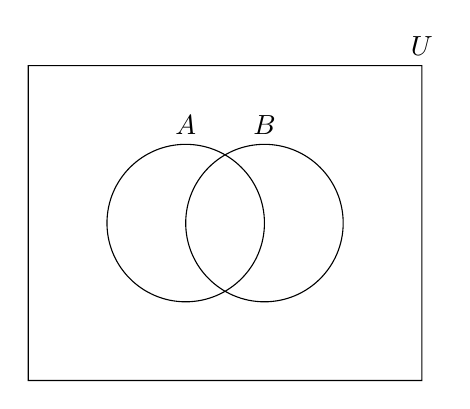
\begin{tikzpicture}[fill=white]
    \draw (0,0) circle (1) (0,1)  node [text=black,above] {$A$}
    (1,0) circle (1) (1,1)  node [text=black,above] {$B$}
    (-2,-2) rectangle (3,2) node [text=black,above] {$U$};
  \end{tikzpicture}
\end{center}

If $A \subseteq B$ and there is an element of $B$ that is not an element of $A$, meaning $A \not = B$,
then $A$ is a \textbf{proper subset} of $B$, denoted as $A \subset B$. An important fact is that
$\mathbb{N} \subset \mathbb{Z} \subset \mathbb{B} \subset \mathbb{R}$

\subsection{Sets of sets}

Elements of sets can be sets themselves, consider $A = \{\{1, 2\}, \emptyset, \{1, 2, 3\}, \{1\}\}$.
The cardinality of $A$ is 4, $\left\lvert A\right\rvert = 4$. Additionally, $\{1, 2\} \in A$, but
$1 \not \in A$.

The \textbf{Powerset} of A, denoted as $P(A)$ is the set of all subsets of $A$. For example,
\begin{align*}
  A    & = \{1, 2, 3\}                                                        \\
  P(A) & = \{\{1\}, \{2\}, \{3\}, \{1, 2\}, \{1, 3\}, \{2, 3\}, \{1, 2, 3\}\}
\end{align*}

\subsubsection*{Cardinality of a Powerset}

Let A be a finite set of cardinality $n$. Then the cardinality of the powerset of A is $2^n$.
\begin{align*}
  \left\lvert A\right\rvert    & = n   \\
  \left\lvert P(A)\right\rvert & = 2^n
\end{align*}

\subsection{Union and Intersection}

\textbf{Intersection} set operation: $\cap$.
$A$ intersected with $B$ is defined to be the set containing elements which are in both $A$ \underline{and} $B$.
That is, $A \cap B = \{x: x \in A \land x \in B\}$.
\begin{center}
  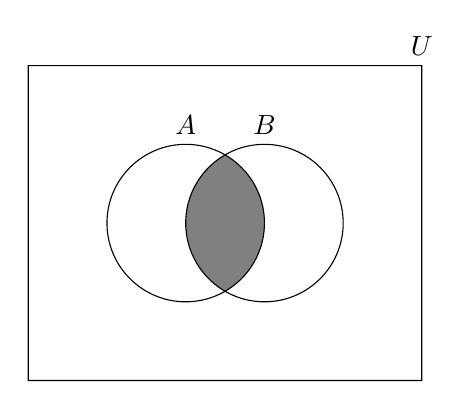
\begin{tikzpicture}
    \filldraw[fill=white] (-2,-2) rectangle (3,2);
    \scope % A \cap B
    \clip (0,0) circle (1);
    \fill[gray] (1,0) circle (1);
    \endscope
    % outline
    \draw (0,0) circle (1) (0,1)  node [text=black,above] {$A$}
    (1,0) circle (1) (1,1)  node [text=black,above] {$B$}
    (-2,-2) rectangle (3,2) node [text=black,above] {$U$};
  \end{tikzpicture}
\end{center}

Intersection $\cap$ can also apply to infinite sets:
\begin{align*}
  A        & =\{x \in \mathbb{Z}: x \text{ is an integer multiple of 2}\}  \\
  B        & =\{x \in \mathbb{Z}: x \text{ is an integer multiple of 3}\}  \\
  A \cap B & = \{x \in \mathbb{Z}: x \text{ is an integer multiple of 6}\}
\end{align*}

\noindent \textbf{Union} set operation $\cup$.
$A$ union with $B$ is defined to be the set containing elements which are in $A$ \underline{or} $B$.
That is, $A \cup B = \{x: x \in A \lor x \in B\}$.
\begin{center}
  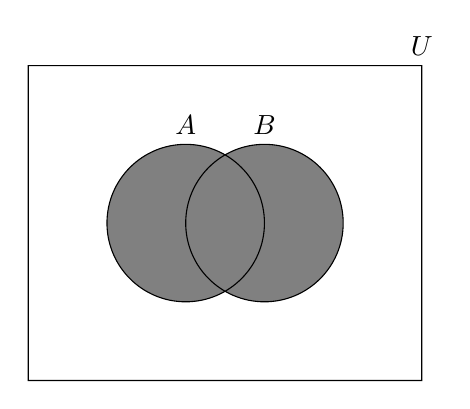
\begin{tikzpicture}
    \filldraw[fill=white] (-2,-2) rectangle (3,2);
    \fill[gray] (0,0) circle (1);
    \fill[gray] (1,0) circle (1);
    % outline
    \draw (0,0) circle (1) (0,1)  node [text=black,above] {$A$}
    (1,0) circle (1) (1,1)  node [text=black,above] {$B$}
    (-2,-2) rectangle (3,2) node [text=black,above] {$U$};
  \end{tikzpicture}
\end{center}

A special notation, similar to $\sum$ or $\prod$ notation, allows for compound representation of the
intersections or unions of a long sequence of sets.
\begin{align*}
  \bigcap_{i=1}^{n} A_{i} & = A_1 \cap A_2 \cap A_3 \cap \cdots \cap A_n = \{x : x \in A, \text{ for \underline{all} } 1 \leq i \leq n\}  \\
  \bigcup_{i=1}^{n} A_{i} & = A_1 \cup A_2 \cup A_3 \cup \cdots \cup A_n = \{x : x \in A, \text{ for \underline{some} } 1 \leq i \leq n\} \\
\end{align*}

Consider $A_j =$ a word with $j$ letters, with $U =$ is the Oxford English Dictionary.
\begin{align*}
  \bigcup_{j=1}^{10} A_j & = \text{ the set of all words with 10 letters or fewer in the OED} \\
  \bigcap_{j=1}^{45} A_j & = \emptyset                                                        \\
  \bigcup_{j=1}^{45} A_j & = \text{ the set of all words in the OED.}
\end{align*}

\subsection{More set operations}

\textbf{Difference} set operation $-$.
$A$ difference with $B$ is defined to be the set containing elements which are in $A$ but \underline{not} $B$.
That is, $A - B = \{x: x \in A \land x \not \in B\}$. A set difference is \underline{not} strictly commutative, often
$A - B \not = B - A$.
\begin{center}
  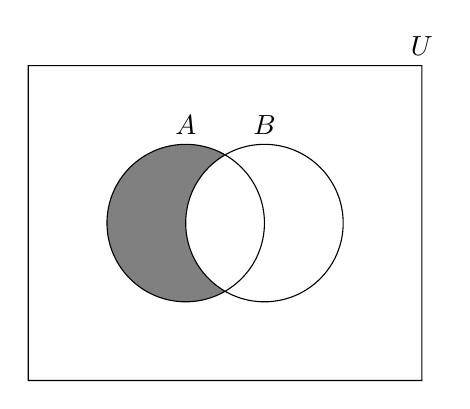
\begin{tikzpicture}[fill=gray]
    % left hand
    \scope
    \clip (-2,-2) rectangle (2,2)
    (1,0) circle (1);
    \fill (0,0) circle (1);
    \endscope
    % outline
    \draw (0,0) circle (1) (0,1)  node [text=black,above] {$A$}
    (1,0) circle (1) (1,1)  node [text=black,above] {$B$}
    (-2,-2) rectangle (3,2) node [text=black,above] {$U$};
  \end{tikzpicture}
\end{center}

\noindent \textbf{Symmetric Difference} set operation $\triangle$.
$A$ symmetric difference with $B$ is defined to be the set containing elements which are in $A$ or $B$, but not $A$ and $B$.
That is, $A \triangle B = \{x: x \in A \oplus  x \in B\}$.
\begin{center}
  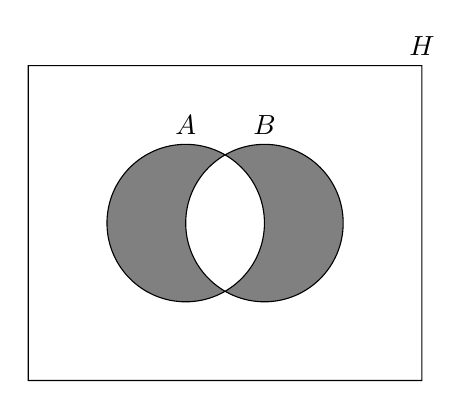
\begin{tikzpicture}[fill=gray]
    % left hand
    \scope
    \clip (-2,-2) rectangle (2,2)
    (1,0) circle (1);
    \fill (0,0) circle (1);
    \endscope
    % right hand
    \scope
    \clip (-2,-2) rectangle (2,2)
    (0,0) circle (1);
    \fill (1,0) circle (1);
    \endscope
    % outline
    \draw (0,0) circle (1) (0,1)  node [text=black,above] {$A$}
    (1,0) circle (1) (1,1)  node [text=black,above] {$B$}
    (-2,-2) rectangle (3,2) node [text=black,above] {$H$};
  \end{tikzpicture}
\end{center}

\noindent \textbf{Complement} set operation $\overline{ }$.
complement $A$ is defined to be the set containing elements in $U$ which are not in $A$.
That is, $\overline{A}= \{x: x \in U \land x \not \in A\}$.
\begin{center}
  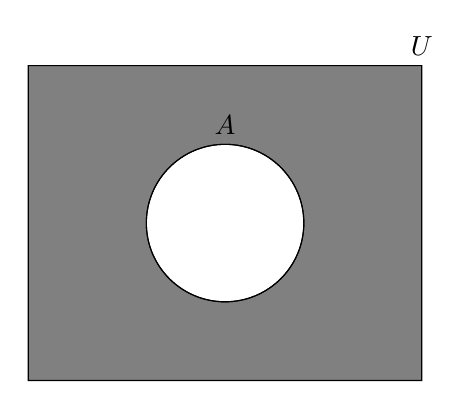
\begin{tikzpicture}[fill=white]
    \draw[fill=gray] (-2,-2) rectangle (3,2);
    \draw[fill=white] (0.5,0) circle (1);
    % outline
    \draw (0.5,0) circle (1) (0.5,1)  node [text=black,above] {$A$}
    (-2,-2) rectangle (3,2) node [text=black,above] {$U$};
  \end{tikzpicture}
\end{center}

\begin{center}
  \begin{tabular}{l|c|l}
    \multicolumn{3}{c}{\textbf{Summary of Set Operations}}                       \\
    Operation            & Notation        & Set Builder                         \\
    \hline
    Intersection         & $A \cap B$      & $\{x: x \in A \land x \in B\}$      \\
    Union                & $A \cup B$      & $\{x: x \in A \lor x \in B\}$       \\
    Difference           & $A - B$         & $\{x: x \in A \land x \not \in B\}$ \\
    Symmetric Difference & $A \triangle B$ & $\{x: x \in A \oplus  x \in B\}$    \\
    Complement           & $\overline{A}$  & $\{x: x \in U \land x \not \in A\}$ \\
  \end{tabular}
\end{center}

\subsection{Set identities}

The laws of propositional logic can be used to derive corresponding set identities.
A \textbf{set identity} is an equation involving sets that is true,
regardless of the contents of the sets used in the expression.
\begin{center}
  \begin{tabular}{r|c|c}
    \textbf{Law Name} & $\cup$ Union                                           & $\cap$ Intersection                                    \\
    \hline
    Idempotent        & $A \cup A = A$                                         & $A \cap A = A$                                         \\
    Associative       & $(A \cup B) \cup C = A \cup (B \cup C)$                & $(A \cap B) \cap C = A \cap (B \cap C)$                \\
    Commutative       & $A \cup B = B \cup A$                                  & $A \cap B = B \cap A$                                  \\
    Distributive      & $A \cup (B \cap C) = (A \cup B) \cap (A \cup C)$       & $A \cap (B \cup C) = (A \cap B) \cup (A \cap C)$       \\
    Identity          & $A \cup \emptyset = A$                                 & $A \cap U = A$                                         \\
    Domination        & $A \cup U = U$                                         & $A \cap \emptyset = \emptyset$                         \\
    Double Complement & $\overline{\overline{A}} = A$                                                                                   \\
    Complement        & $A \cup \overline{A} =$ T                              & $A \cap \overline{A} =$ F                              \\
    DeMorgan          & $\overline{A \cup B} = \overline{A} \cap \overline{B}$ & $\overline{A \cap B} = \overline{A} \cup \overline{B}$ \\
    Absorption        & $A \cup (A \cap B) = A$                                & $A \cap (A \cup B) = A$
  \end{tabular}
\end{center}

\subsection{Cartesian products}

An \textbf{ordered pair} of items is written $(x, y)$, where the first entry is $x$ and the second entry is $y$.
The use of $()$ instead of $\{\}$ indicates that order matters.

\noindent \textbf{Cartesian Product} of $A$ and $B$, $A \times B = \{(a, b) : a \in A \land b \in B\}$
\begin{align*}
  A & = \{1, 2\}    & A \times B & = \{(1, a), (1, b), (1, c), (2, a), (2, b), (2, c)\} \\
  B & = \{a, b, c\} & B \times A & = \{(a, 1), (a, 2), (b, 1), (b, 2), (c, 1), (c, 2)\}
\end{align*}

An ordered list of 3 items is called an \textbf{ordered triple}, denoted as $(x, y, z)$.
For a size of $\geq 4$, use the term \textbf{n-tuple}. For example, $(u, w, x, y, z)$.
\begin{align*}
  A_1 \times A_2 \times \cdots \times A_n = \{(a_1, a_2, \ldots, a_n) : a_i \in A \text{ for all $i$ such that} 1 \leq i \leq n\}
\end{align*}
Another Example
\begin{align*}
  A & = \{a, b\}          & (a, 1, y, \beta)  & \in A \times B \times C \times D      \\
  B & = \{1, 2\}          & (b, 1, x, \alpha) & \in A \times B \times C \times D      \\
  C & = \{x, y\}          & (1, b, x, \beta)  & \not \in A \times B \times C \times D \\
  D & = \{\alpha, \beta\} &                   & \text{order matters}
\end{align*}

$A \times A = A^2$, and in general,
\begin{align*}
  A^k = \underbrace{A \times A \times \cdots \times A}_{k-times}
\end{align*}
The \textbf{Cardinality of Cartesian Products}:
\begin{align*}
  \left\lvert A^n \right\rvert                           & = {\left\lvert A \right\rvert}^n                                               \\
  \left\lvert A_1 \times A_2 \times \cdots  \right\rvert & = \left\lvert A_1 \right\rvert \cdot \left\lvert A_2 \right\rvert \cdot \cdots
\end{align*}

\subsubsection*{Strings}

A sequence of characters is called a \textbf{string}.
The set of characters used in a set of string is called the \textbf{alphabet} for the set of strings.
The \textbf{length} of a string is the number of characters in the string.
For example, the length of $'xxyxyx'$ is $6$.
The \textbf{empty string} is a string whose length is $0$, and is usually denoted by $\lambda$.
It is useful for $A^0$, for some alphabet $A$. $\{0, 1\}^0 = \{\lambda\}$.
If $s$ and $t$ are two strings, then the \textbf{concatenation} of $s$ and $t$ is the string obtained by putting $s$ and $t$ together.
\begin{align*}
  s & = 010 & st & = 01011 \\
  t & = 11  & t0 & = 110
\end{align*}
Strings are used to specify passwords for computers or online accounts.
Security systems vary with respect to the alphabet of characters allowed or required in a valid password.
Strings also play an important rules in discrete mathematics as a mathematical tool to help count cardinality of sets.

\subsection{Partitions}

Two sets, $A$ and $B$, are said to be \textbf{disjoint} if their intersection is empty $(A \cap B = \emptyset)$.
A sequence of sets, $A_1, A_2, A_3, \ldots, A_n$, is \textbf{pairwise disjoint} if every pair of distinct sets in the sequence is disjoint.
A \textbf{partition} of a non-empty set $A$ is a collection of non-empty subsets such that each element of $A$ is in exactly one of the subsets.
$A_1, A_2, A_3, \ldots, A_n$ is a partition for a nonempty set $A$ if:
\begin{itemize}
  \item For all $i, A_i \subseteq A$
  \item For all $i, A_i \not = \emptyset$
  \item $A_1, A_2, \ldots, A_n$ are pairwise disjoint
  \item $A = \bigcup_{i=1}^{n} A_i$, for some $n \in \mathbb{Z}^+$
\end{itemize}
\begin{center}
  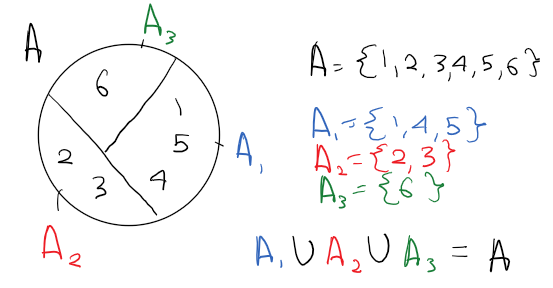
\includegraphics[width=.6\linewidth]{resources/partitions.png}
\end{center}
\section{Functions}
\subsection{Definition of functions}

A \textbf{function} maps elements of one set $X$ to elements of another set $Y$.
A function from $X$ to $Y$ can be viewed as a subset of $X \times Y : (x, y) \in f$ if $f$ maps $x$ to $y$.
The notation for a function is:
\[
  f: X \rightarrow Y \text{, where $X$ is the \textbf{domain} and $Y$ is the \textbf{co-domain}.}
\]

*if $f$ maps an element of the domain to zero elements \underline{or} more than one element of the target,
then $f$ is \underline{not} \textit{well-defined}

\textbf{Arrow Diagram}:
\begin{align*}
  X & = \{w, x, y, z\} \\
  Y & = \{a, b, c, d\}
\end{align*}

Well-defined functions:
\begin{center}
  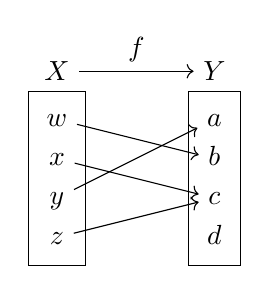
\begin{tikzpicture}
    \foreach[count=\i] \set/\elements in {X/{w,x,y,z}, Y/{a,b,c,d}} { %domain and co-domain
    \begin{scope}[local bounding box=\set, x=2cm, y=0.5cm]
      \foreach[count=\j] \element in \elements {
        \node[minimum width=1em,anchor=base,text height=1.4ex,text depth=0.25ex]
        (\i-\element) at (\i,-\j) {$\element$};
      }
    \end{scope}
    \node[draw, fit=(\set), label={[name=\i]above:$\set$}] {};
    }
    \foreach \domain/\target in {w/b,x/c,y/a,z/c} { %function pairs, uses indices
        \draw[->] (1-\domain) -- (2-\target);
      }
    \draw[->] (1) -- node[above]{$f$}(2); %function name
  \end{tikzpicture}
  \qquad
  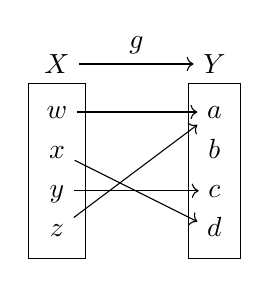
\begin{tikzpicture}
    \foreach[count=\i] \set/\elements in {X/{w,x,y,z}, Y/{a,b,c,d}} { %domain and co-domain
    \begin{scope}[local bounding box=\set, x=2cm, y=0.5cm]
      \foreach[count=\j] \element in \elements {
        \node[minimum width=1em,anchor=base,text height=1.4ex,text depth=0.25ex]
        (\i-\element) at (\i,-\j) {$\element$};
      }
    \end{scope}
    \node[draw, fit=(\set), label={[name=\i]above:$\set$}] {};
    }
    \foreach \domain/\target in {w/a,x/d,y/c,z/a} { %function pairs, uses indices
        \draw[->] (1-\domain) -- (2-\target);
      }
    \draw[->] (1) -- node[above]{$g$}(2); %function name
  \end{tikzpicture}
\end{center}

\underline{Not} well-defined functions:
\begin{center}
  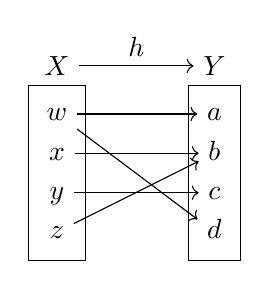
\begin{tikzpicture}
    \foreach[count=\i] \set/\elements in {X/{w,x,y,z}, Y/{a,b,c,d}} { %domain and co-domain
    \begin{scope}[local bounding box=\set, x=2cm, y=0.5cm]
      \foreach[count=\j] \element in \elements {
        \node[minimum width=1em,anchor=base,text height=1.4ex,text depth=0.25ex]
        (\i-\element) at (\i,-\j) {$\element$};
      }
    \end{scope}
    \node[draw, fit=(\set), label={[name=\i]above:$\set$}] {};
    }
    \foreach \domain/\target in {w/a,w/d,x/b,y/c,z/b} { %function pairs, uses indices
        \draw[->] (1-\domain) -- (2-\target);
      }
    \draw[->] (1) -- node[above]{$h$}(2); %function name
  \end{tikzpicture}
  \qquad
  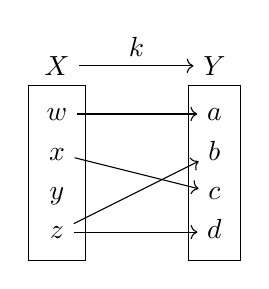
\begin{tikzpicture}
    \foreach[count=\i] \set/\elements in {X/{w,x,y,z}, Y/{a,b,c,d}} { %domain and co-domain
    \begin{scope}[local bounding box=\set, x=2cm, y=0.5cm]
      \foreach[count=\j] \element in \elements {
        \node[minimum width=1em,anchor=base,text height=1.4ex,text depth=0.25ex]
        (\i-\element) at (\i,-\j) {$\element$};
      }
    \end{scope}
    \node[draw, fit=(\set), label={[name=\i]above:$\set$}] {};
    }
    \foreach \domain/\target in {w/a,x/c,z/b,z/d} { %function pairs, uses indices
        \draw[->] (1-\domain) -- (2-\target);
      }
    \draw[->] (1) -- node[above]{$k$}(2); %function name
  \end{tikzpicture}
\end{center}

For function $f: X \rightarrow Y$, an element $y$ is in the \textbf{range} of $f$
iff there is an $x \in X$ such that $(x, y) \in f$.
\[
  \text{Range of } f = \{y : (x, y) \in f, \text{ for some } x \in X\}
\]
Two functions, $f$ and $g$, are \textbf{equal} if $f$ and $g$ have the same domain and target and
$f(x) = g(x)$ for \underline{every} $x$ in the domain.
\[
  \forall~ x : f(x) = g(x) \implies f = g
\]

\subsection{Floor and Ceiling functions}

The \textbf{Floor} function, $\left\lfloor x\right\rfloor$
\[
  \text{floor}: \mathbb{R} \rightarrow \mathbb{Z}, \text{ where floor$(x)$ = the largest integer $y$ such that $y \leq x$.}
\]
Notation: $\text{floor}(x) = \left\lfloor x\right\rfloor$
\[\]
\noindent The \textbf{Ceiling} function, $\left\lceil x\right\rceil$
\[
  \text{ceiling}: \mathbb{R} \rightarrow \mathbb{Z}, \text{ where ceiling$(x)$ = the smallest integer $y$ such that $y \geq x$.}
\]
Notation: $\text{ceiling}(x) = \left\lceil x\right\rceil$

\noindent Examples of floor and ceiling:
\begin{align*}
  \left\lceil 4.32\right\rceil  & = 5  & \left\lfloor 4.32\right\rfloor  & = 4  \\
  \left\lceil -4.32\right\rceil & = -4 & \left\lfloor -4.32\right\rfloor & = -5 \\
  \left\lceil 4\right\rceil     & = 4  & \left\lfloor 4\right\rfloor     & = 4  \\
  \left\lceil -4\right\rceil    & = -4 & \left\lfloor -4\right\rfloor    & = -4 \\
\end{align*}

\subsection{Properties of functions}

A function $f: X \rightarrow Y$ is \textbf{one-to-one} or \textbf{injective} if $x_1 \not = x_2$ implies that $f(x_1) \not = f(x_2)$.
$f$ maps different elements in x to different elements in y.

A function $f: X \rightarrow Y$ is \textbf{onto} or \textbf{surjective} if the range of $f$ is equal to the target $Y$.
That is, $\forall~ y \exists~ x (y \in Y \land x \in X \land f(x) = y)$

A function $f: X \rightarrow Y$ is \textbf{bijective} if it is both \textbf{injective} and \textbf{surjective}.
A \textbf{bijective} function is called a \textbf{bijection}, or a \textbf{one-to-one correspondence}.

When the domain and target are finite sets, it is possible to infer information about their relative sizes
based on whether a function is one-to-one or onto.
\begin{align*}
  f: D \rightarrow T & \text{ is \textbf{one-to-one}} & \implies &  & \left\lvert D\right\rvert & \leq \left\lvert T\right\rvert \\
  f: D \rightarrow T & \text{ is \textbf{onto}}       & \implies &  & \left\lvert D\right\rvert & \geq \left\lvert T\right\rvert \\
  f: D \rightarrow T & \text{ is \textbf{bijective}}  & \implies &  & \left\lvert D\right\rvert & = \left\lvert T\right\rvert
\end{align*}

\subsection{The inverse of a function}

If a function $f: X \rightarrow Y$ is a \textit{bijection},
then the \textbf{inverse} of f is obtained by exchanging the first and second entries in each pair in $f$.
\begin{align*}
  \text{given } f        & : X \rightarrow Y           \\
  \text{inverse } f^{-1} & : \{(y, x) : (x, y) \in f\}
\end{align*}
Reversing the cartesian pair does not always create a well-defined function.
\textit{Some functions do not have an inverse}.

\textbf{Examples}:
\begin{align*}
  X & = \{1, 2, 3\} & f = \{(1, 7), (2, 9), (3, 9)\} \\
  Y & = \{7, 8, 9\} & g = \{(1, 9), (2, 7), (3, 8)\}
\end{align*}

\begin{center}
  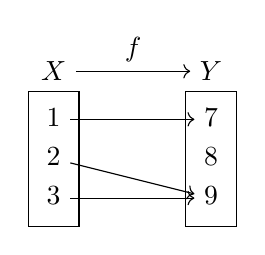
\begin{tikzpicture}
    \foreach[count=\i] \set/\elements in {X/{1,2,3}, Y/{7,8,9}} { %domain and co-domain
    \begin{scope}[local bounding box=\set, x=2cm, y=0.5cm]
      \foreach[count=\j] \element in \elements {
        \node[minimum width=1em,anchor=base,text height=1.4ex,text depth=0.25ex]
        (\i-\element) at (\i,-\j) {$\element$};
      }
    \end{scope}
    \node[draw, fit=(\set), label={[name=\i]above:$\set$}] {};
    }
    \foreach \domain/\target in {1/7,2/9,3/9} { %function pairs, uses indices
        \draw[->] (1-\domain) -- (2-\target);
      }
    \draw[->] (1) -- node[above]{$f$}(2); %function name
  \end{tikzpicture}
  \qquad
  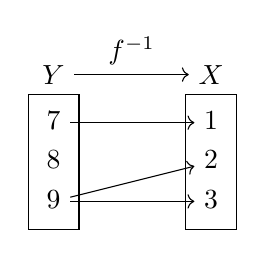
\begin{tikzpicture}
    \foreach[count=\i] \set/\elements in {Y/{7,8,9}, X/{1,2,3}} { %domain and co-domain
    \begin{scope}[local bounding box=\set, x=2cm, y=0.5cm]
      \foreach[count=\j] \element in \elements {
        \node[minimum width=1em,anchor=base,text height=1.4ex,text depth=0.25ex]
        (\i-\element) at (\i,-\j) {$\element$};
      }
    \end{scope}
    \node[draw, fit=(\set), label={[name=\i]above:$\set$}] {};
    }
    \foreach \domain/\target in {7/1,9/2,9/3} { %function pairs, uses indices
        \draw[->] (1-\domain) -- (2-\target);
      }
    \draw[->] (1) -- node[above]{$f^{-1}$}(2); %function name
  \end{tikzpicture}

  $f^{-1}$ is not well defined, therefore $f$ does not have an inverse.
\end{center}
\begin{center}
  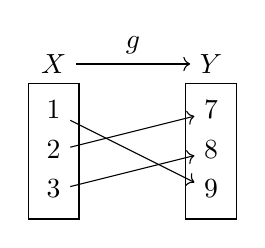
\begin{tikzpicture}
    \foreach[count=\i] \set/\elements in {X/{1,2,3}, Y/{7,8,9}} { %domain and co-domain
    \begin{scope}[local bounding box=\set, x=2cm, y=0.5cm]
      \foreach[count=\j] \element in \elements {
        \node[minimum width=1em,anchor=base,text height=1.4ex,text depth=0.25ex]
        (\i-\element) at (\i,-\j) {$\element$};
      }
    \end{scope}
    \node[draw, fit=(\set), label={[name=\i]above:$\set$}] {};
    }
    \foreach \domain/\target in {1/9,2/7,3/8} { %function pairs, uses indices
        \draw[->] (1-\domain) -- (2-\target);
      }
    \draw[->] (1) -- node[above]{$g$}(2); %function name
  \end{tikzpicture}
  \qquad
  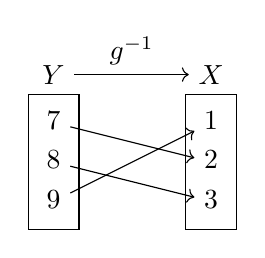
\begin{tikzpicture}
    \foreach[count=\i] \set/\elements in {Y/{7,8,9}, X/{1,2,3}} { %domain and co-domain
    \begin{scope}[local bounding box=\set, x=2cm, y=0.5cm]
      \foreach[count=\j] \element in \elements {
        \node[minimum width=1em,anchor=base,text height=1.4ex,text depth=0.25ex]
        (\i-\element) at (\i,-\j) {$\element$};
      }
    \end{scope}
    \node[draw, fit=(\set), label={[name=\i]above:$\set$}] {};
    }
    \foreach \domain/\target in {9/1,7/2,8/3} { %function pairs, uses indices
        \draw[->] (1-\domain) -- (2-\target);
      }
    \draw[->] (1) -- node[above]{$g^{-1}$}(2); %function name
  \end{tikzpicture}

  $g^{-1}$ is well defined, therefore $g$ does have an inverse.
\end{center}

\subsection{Composition of functions}

The process of applying a function to the result of another function is called \textbf{composition}.
\begin{align*}
  f           & : X \rightarrow Y                                                                   \\
  g           & : Y \rightarrow Z                                                                   \\
  (g \circ f) & : X \rightarrow Z, \text{ such that } \forall~ x : x \in X, (g \circ f)(x) = g(f(x))
\end{align*}
Remember that order matters, as often $(g \circ f)(x) \not = (f \circ g)(x)$. However, composition is associative:
\[
  (f \circ g \circ h)(x) = ((f \circ g) \circ h)(x) = (f \circ (g \circ h))(x) = f(g(h(x)))
\]

\subsubsection*{Identity Function}

The \textbf{Identity Function} maps a set onto itself and maps every element to itself. It is notated as $I_A: A \rightarrow A$,
where $A$ is the set it maps. There are a number of identities about the Identity Function.

Let $f: A \rightarrow B$ be a bijection. Then,
\[
  f \circ f^{-1} = I_B \text{ and } f^{-1} \circ f = I_A
\]

\subsection{Logarithms and exponents}

The \textbf{Exponential} function, $\text{exp}_b: \mathbb{R} \rightarrow \mathbb{R}^+, \text{exp}_b(x) = b^x$.
$b$ is the base of the exponent and $x$ is the exponent.

Properties of exponents:
\begin{align*}
  b^{x}b^{y}      & = b^{x+y} & b & \in \mathbb{R}^+ & c & \in \mathbb{R}^+ \\
  (b^x)^{y}       & = b^{xy}  & x & \in \mathbb{R}   & y & \in \mathbb{R}   \\
  \frac{b^x}{b^y} & = b^{x-y}                                               \\
  (bc)^x          & = b^xc^x
\end{align*}

\begin{center}
  \begin{tikzpicture}
    \draw[<->] (-3,0) -- (3,0) node[right] {$x$};
    \draw[<->] (0,-3) -- (0,3) node[above] {$y$};
    \begin{scope}
      \clip (-3,-3) rectangle (3,3);
      \draw[domain=-3:3, variable=\x, samples=50, smooth, blue, thick] plot ({\x}, {(exp(\x))});
    \end{scope}
    \begin{scope}
      \clip (-3,-3) rectangle (3,3);
      \draw[domain=0.0001:3, variable=\x, samples=50, smooth, red, thick] plot ({\x}, {(ln(\x))});
    \end{scope}
    \draw (-1,-1) node[red] {log$(x)$};
    \draw (2,2) node[blue] {exp$(x)$};
  \end{tikzpicture}
\end{center}

The \textbf{Logarithms} function, $\text{log}_b: \mathbb{R} \rightarrow \mathbb{R}^+, \text{log}_b(y) = x$.
$b$ is the base of the logarithm and $x$ is the exponent.

Properties of exponents:
\begin{align*}
  \text{log}_b(xy)          & = \text{log}_bx + \text{log}_by       & b & \in \mathbb{R}^+ \\
  \text{log}_b(\frac{x}{y}) & = \text{log}_bx - \text{log}_by       & c & \in \mathbb{R}^+ \\
  \text{log}_b(x^y)         & = y\text{log}_bx                      & x & \in \mathbb{R}   \\
  \text{log}_cx             & = \frac{\text{log}_bx}{\text{log}_bc} & y & \in \mathbb{R}
\end{align*}
\section{Boolean Algebra}
\subsection{An introduction to Boolean Algebra}

\textbf{Boolean Algebra} is a set of rules/operations for working with variables whose values are either 0 or 1.
It corresponds highly to propositional logic.

\textbf{Boolean Multiplication}, denoted by $\cdot$.
\begin{align*}
  \text{Boolean } & \cdot & \text{Logic }           & \land      \\
  0 \cdot 0       & = 0   & \text{F} \land \text{F} & = \text{F} \\
  0 \cdot 1       & = 0   & \text{F} \land \text{T} & = \text{F} \\
  1 \cdot 0       & = 0   & \text{T} \land \text{F} & = \text{F} \\
  1 \cdot 1       & = 1   & \text{T} \land \text{T} & = \text{T}
\end{align*}

\textbf{Boolean Addition}, denoted by $+$.
\begin{align*}
  \text{Boolean } & \cdot & \text{Logic }          & \lor       \\
  0 + 0           & = 0   & \text{F} \lor \text{F} & = \text{F} \\
  0 + 1           & = 1   & \text{F} \lor \text{T} & = \text{T} \\
  1 + 0           & = 1   & \text{T} \lor \text{F} & = \text{T} \\
  1 + 1           & = 1   & \text{T} \lor \text{T} & = \text{T} \\
\end{align*}

\textbf{Boolean Complement}, denoted by $\bar{ }$.
\begin{align*}
  \text{Boolean } & \bar{ } & \text{Logic }  & \lnot      \\
  \bar{0}         & = 1     & \lnot \text{F} & = \text{T} \\
  \bar{1}         & = 0     & \lnot \text{T} & = \text{F} \\
\end{align*}

\begin{center}
  \begin{circuitikz}
    \draw (0,0) to[battery] (0,2)
    to[switch, l=$x$] (2,2)
    to[switch, l=$y$](4,2)
    to[lamp] (4,0) -- (0,0);
    \draw (2,-1) node[] {Shannon Circuit (AND $\cdot$)};
  \end{circuitikz}
  \qquad
  \begin{circuitikz}
    \draw (0,0) to[battery] (0,2) -- (1,2) -- (1,1.5)
    to[switch, l=$x$] (3,1.5) -- (3,2) -- (4,2) to[lamp] (4,0) -- (0,0)
    (1,2) -- (1,2.5)
    to[switch, l=$y$] (3,2.5) -- (3,2);
    \draw (2,-1) node[] {Switching Circuit (OR $+$)};
  \end{circuitikz}
\end{center}

Variables that can have a value of either $1$ or $0$ are called \textbf{Boolean Variables}.
Boolean expressions are made of boolean variables. There are also common shorthand ways of notating operations.
\begin{align*}
  x \cdot y + 1 \cdot \bar{z} & = xy + \bar{z}        \\
  x + z + \overline{0 + y}    & = x + z \cdot \bar{y}
\end{align*}

\begin{center}
  \begin{tabular}{r|c|c}
    \textbf{Law Name} & $+$ OR                                               & $\cdot$ AND                                          \\
    \hline
    Idempotent        & $x + x = x$                                          & $x \cdot x = x$                                      \\
    Associative       & $(x + y) + z = x + (y + z)$                          & $(x \cdot y) \cdot z = x \cdot (y \cdot z)$          \\
    Commutative       & $x + y = y + x$                                      & $x \cdot y = y \cdot x$                              \\
    Distributive      & $x + (y \cdot z) = (x + y) \cdot (x + z)$            & $x \cdot (y + z) = (x \cdot y) + (x \cdot z)$        \\
    Identity          & $x + 0 = x$                                          & $x \cdot 1 = x$                                      \\
    Domination        & $x + 1 = 1$                                          & $x \cdot 0 = 0$                                      \\
    Double Complement & $\overline{\overline{x}} = x$                                                                               \\
    Complement        & $x + \overline{x} =$ 1                               & $x \cdot \overline{x} =$ 0                           \\
    DeMorgan          & $\overline{x + y} = \overline{x} \cdot \overline{y}$ & $\overline{x \cdot y} = \overline{x} + \overline{y}$ \\
    Absorption        & $x + (x \cdot y) = x$                                & $x \cdot (x + y) = x$
  \end{tabular}
\end{center}

\subsection{Boolean functions}
\subsection{Disjunctive and conjunctive normal form}
\subsection{Functional completeness}
\subsection{Boolean satisfiability}
\subsection{Gates and circuits}
\section{Relation and Digraphs}
\subsection{Introduction to binary relations}
\subsection{Properties of binary relations}
\subsection{Directed graphs, paths, and cycles}
\subsection{Composition of relations}
\subsection{Graph powers and the transitive closure}
\subsection{Matrix multiplication and graph powers}
\subsection{Partial orders}
\subsection{Strict orders and directed acyclic graphs}
\subsection{Equivalence relations}
\subsection{N-ary relations and relational databases}
\section{Computation}
\subsection{An introduction to algorithms}
\subsection{Asymptotic growth of functions}
\subsection{Analysis of algorithms}
\subsection{Finite state machines}
\subsection{Turing machines}
\subsection{Decision problems and languages}
\section{Induction and Recursion}
\subsection{Sequences}
A \textbf{sequence} is a special type of function in which the domain
is the set of consecutive integers.

When a function is specified as a sequence, using subscripts to denote input
is more common, so $g_k$ is used instead of $g(k)$

A value $g_k$ is called a \textbf{term}, and $k$ is the \textit{index} of $g_k$

For example:
\begin{align*}
  g_1 & = 3.67 & g_2 & = 2.88 \\
  g_3 & = 3.25 & g_4 & = 3.75
\end{align*}
\[
  g(k) = 3.67, 2.88, 3.25, 3.75
\]

An entire sequence is denoted by $\{gk\}$, whereas $g_k$ is used to denote a
single term in the sequence.

A sequence commonly starts with $0$ or $1$, but it could be \textit{any} integer.
\subsubsection*{Finite sequence}
A sequence with a finite domain is a \textbf{finite sequence}.
In a finite sequence, there is an \textit{initial index $m$} and a \textit{final index $n$}.
\subsubsection*{Infinite sequence}
A sequence with an infinite domain is a \textbf{infinite sequence}.
In an infinite sequence, there is an \textit{initial index m} and the sequence
is defined for indices $k \geq m$:
\[
  a_m, a_{m+1}, a_{m+2}, a_{m+3}, \ldots
\]
A sequence can be specified by an \textbf{explicit formula}, such as $d_k = 2^k$
for $k \geq 1$.
\[
  \{d_k\} = 2,4,8,16, \ldots
\]
\subsubsection*{Increasing and Decreasing Sequences}
\begin{itemize}
  \item a sequence is \textit{increasing} if for every two consecutive indices, $k$
        and $k+1$, $a_k < a_{k+1}$
  \item a sequence is \textit{non-decreasing} if for every two consecutive indices, $k$
        and $k+1$, $a_k \leq a_{k+1}$
\end{itemize}
For example,
\begin{align*}
  2 < 4 < 5 < 6          & ~\text{increasing \textit{and} non-decreasing}     \\
  2 \leq 4 \leq 5 \leq 6 & ~\text{non-decreasing \textit{but} not increasing}
\end{align*}
\textit{The same relationship can be said for \textbf{decreasing} and \textbf{non-increasing}}.
\subsubsection*{Geometric Sequences}
A \textbf{geometric sequence} is a sequence of real numbers where each term is found by taking
the previous term and multiplying it by a fixed number called the \textbf{common ratio}.

For example, with an \textit{initial term}: 4, and \textit{common ratio}: $\frac{1}{2}$,
\[
  4,2,\frac{1}{2},\frac{1}{4}, \ldots
\]
\subsubsection*{Arithmetic Sequence}
An \textbf{arithmetic sequence} is a sequence of real numbers where each term after the initial
term is found by taking the previous term and adding a fixed number called the \textbf{common difference}.

For example, with an \textit{initial value}: 2, and \textit{common difference}: 3,
\[
  2,5,8,11, \ldots
\]

\subsection{Recurrence relations}
A rule that defines a term $a_n$ as a function of previous terms in the sequence is called a
\textbf{recurrence relation}

For example,
\begin{align*}
  a_0 & = a~\text{initial value} \\
  a_n & = d + a_{n-1}
\end{align*}
Fibonacci Sequence:
\begin{align*}
  f_0 & = 0                                     \\
  f_1 & = 1                                     \\
  f_n & = f_{n-1} + f_{n-2}~\text{for}~n \geq 2 \\
\end{align*}
A \textbf{dynamical system} is a system that changes over time. The state of the system
at any point is determined by a set of well-defined rules that depend on the past states
of the system.

\subsection{Summations}


\subsection{Mathematical induction}


\subsection{More inductive proofs}


\subsection{Strong induction and well-ordering}


\subsection{Loop invariants}


\subsection{Recursive definitions}


\subsection{Structural induction}


\subsection{Recursive algorithms}


\subsection{Induction and recursive algorithms}


\subsection{Analyzing the time complexity of recursive algorithms}


\subsection{Divide-and-conquer algorithms: Introduction and mergesort}


\subsection{Divide-and-conquer algorithms: Binary Search}


\subsection{Solving linear homogeneous recurrence relations}


\subsection{Solving linear non-homogeneous recurrence relations}


\subsection{Divide-and-conquer recurrence relations}

\section{Integer Properties}
\subsection{The Division Algorithm}
\subsection{Modular arithmetic}
\subsection{Prime factorizations}
\subsection{Factoring and primality testing}
\subsection{Greatest common factor divisor and Euclid's algorithm}
\subsection{Number representation}
\subsection{Fast exponentiation}
\subsection{Introduction to cryptography}
\subsection{The RSA cryptosystem}
\section{Introduction to Counting}
\subsection{Sum and Product Rules}

The two most basic rules of counting are the sum and product rule. The \bld{product rule} provides a way to count sequences.

\subsubsection*{Theorem: The Product Rule}
Let $A_1,A_2,\ldots,A_n$ be finite sets. Then,
\[
  | A_1 \times A_2 \times \cdots \times A_n | = |A_1| \cdot |A_2| \cdots |A_n|
\]

\subsubsection*{Counting Strings}
If $\Sigma$ is a set of characters (called an \bld{alphabet}) then $\Sigma^n$ is the set of all string of length $n$ whose characters come from the set $\Sigma$. The product rule can be applied directly to determine the number of strings of a given length over a finite alphabet:
\[
  |\Sigma^n| = |\underbrace{\Sigma \times \Sigma \times \cdots \Sigma}_{\text{$n$ times}}| = \underbrace{|\Sigma| \cdot |\Sigma| \cdots |\Sigma|}_{\text{$n$ times}} = |\Sigma|^n
\]

\subsubsection*{Theorem: The Sum Rule}
Consider $n$ sets, $A_1, A_2, \ldots, A_n$. If the sets are pairwise disjoint, meaning that $A_i \cap A_j = \emptyset \tfor i \neq i$, then
\[
  |A_1 \cup A_2 \cup \cdots \cup A_n| = |A_1| + |A_2| + \cdots + |A_n|
\]

\subsection{The Bijection Rules}
One way to approach difficult counting problems is to show that the cardinality of the set to be counted is equal to the cardinality of a set that is easy to count. The \bld{bijection rule} says that if there is a bijection from one set to another then the two sets have the same cardinality.

A function $f$ from a set $S$ to a set $T$ is called a bijection if and only if $f$ has a well-defined \itl{inverse}, $f^{-1}$.

\subsubsection*{The Bijection Rule}
Let $S \tand T$ be two finite sets. If there is a bijection from $S \tto T$, then $|S|=|T|$

\subsubsection*{The k-to-1 Rule}
Let $X \tand Y$ be finite sets. The function $f: X \rightarrow Y$ is a \bld{k-to-1 correspondence} if for every $y \in Y$, there are exactly $k$ difference $x \in x$ such that $f(x) = y$.

Suppose there is a k-to-1 correspondence from a finite set $A$ to a finite set $B$. Then
\[
  |B| = \frac{|A|}{k}.
\]

\subsection{The generalized product rule}
The \bld{generalized product rule} says that in selecting an item from a set, if the number of choices at each step does not depend on previous choices made, then the number of items in the set is a product of the number of choices in each step.

\subsubsection*{Generalized Product Rule}
Consider a set $S$ of sequences of $k$ items. Suppose there are:
\begin{itemize}
  \item $n_1$ choices for the first item.
  \item For every possible choice for the first item, there are $n_2$ choice for the second item.
  \item For every possible choice for the first and second items, there are $n_3$ choices for the third item.
  \item $\vdots$
  \item For every possible choice for the first $k-1$ items, there are $n_k$ choices for the $k$-th item.
\end{itemize}
Then $|S| = n_1 \cdot n_2 \cdots n_k$.

\subsection{Counting permutations}
An \bld{r-permutation} is a sequence of $r$ items with \bld{no repetitions}, all taken from the same set. In a sequence, order matters, so $(a,b,c)$ is different from $(b,a,c)$.

\subsubsection*{The number of $r$-permutations from a set with $n$ elements}
Let $r \tand n$ be positive integers with $r \leq n$. The number of $r$-permutations from a set with $n$ elements is denoted by $P(n,r)$:
\[
  P(n,r) = \frac{n!}{(n-r)!} = n(n-1)\cdots(n-r+1)
\]

\subsection{Counting subsets}
A subset of size $r$ is called an \bld{r-subset}. An $r$-subset is sometimes referred to as an \bld{r-combination}. In a subset, order does not matter, so $\{a,b,c\}$ is the same as $\{b,a,c\}$. The counting rules for sequences and subsets are commonly referred to as "\itl{permutations} and \itl{combinations}". The term "combination" is the context of counting is another word for "subset".

\subsubsection*{Counting Subsets: 'n choose r' notation}
The number of ways to select an $r$-subset from a set of size $n$ is:
\[
  \begin{pmatrix}
    n \\ r
  \end{pmatrix} = \frac{n!}{r!(n-r)!}.
\]
$\begin{pmatrix}
    n \\ r
  \end{pmatrix}$ is read as "$n$ choose $r$". The notation $C(n,r)$ is sometimes used for $\begin{pmatrix}
    n \\ r
  \end{pmatrix}$.

We can calculated an expression for $\begin{pmatrix}
    n \\ n-r
  \end{pmatrix}$ by replacing $r$ with $n-r$ in the expression for $\begin{pmatrix}
    n \\ r
  \end{pmatrix}$.
\[
  \begin{pmatrix}
    n \\ n-r
  \end{pmatrix} = \frac{n!}{(n-r)!(n-(n-r))!} = \frac{n!}{(n-r!)r!} =
  \begin{pmatrix}
    n \\ r
  \end{pmatrix}
\]
This is an \bld{identity} for $r$-subsets.

\subsection{Subset and permutation examples}

\subsubsection*{Two different cat selection problems: Subset vs. Permutations}
Consider two closely related counting problems:
\begin{enumerate}
  \item A family goes to the animal shelter to adopt 3 cats. The shelter has 20 different cats from which to select. How many ways are there for the family to their selection?
  \item Three different families go to the animal shelter to adopt a cat. Each family will select one cat. How many ways are there for the families to make their selection? (Note that which family gets which cat matters).
\end{enumerate}
In the first problem, the number is ways to make the selection is $\begin{pmatrix}
    20 \\ 3
  \end{pmatrix}$ because the order in which the cats are selected is not important. The outcome is a 3-subset.

In the second problem, the specific cat selected by each family is important. Additionally, no cat can belong to two families. Thus, the answer is $P(20,3) = 20 \cdot 19 \cdot 18$. The outcome is a 3-permutation.

\subsection{Counting by complement}
\bld{Counting by complement} is a technique for counting the number of elements in a set $S$ that have a property by counting the total number of elements in $S$ and subtracting the number of elements in $S$ that do not have the property.
\[
  |P| = |S| - |\bar{P}|
\]
Suppose we want to count the number of people in a room with red hair. We know that there are 20 people in the room and exactly 12 of them do not have red hair. Then we can deduce that the number of people in the room with red hair is 20 - 12 = 8.

\subsection{Permutations with repetitions}
A \bld{permutation with repetition} is an ordering of a set of items in which some of the items may be identical to each other. To illustrate with a smaller example, there are $3! = 6$ permutations of the letters CAT, because the letters in CAT are all different. However, there are only 3 different ways to scramble the letters in DAD: ADD, DAD, DDA.

\subsubsection*{Formula for Counting Permutations with Repetition}
The number of distinct sequences with $n_1 1's, n_2's, \ldots, n_k k's$, where $n = n_1 + n_2 + \cdots + n_k$ is
\[
  \frac{n!}{n_1!n_2!\cdots n_k!}
\]
The formula for permutations with repetition is derived from repeated use of the formula for counting r-subsets:
\begin{align*}
    & \begin{pmatrix}
        n \\ n_1
      \end{pmatrix} \begin{pmatrix}
                      n-n_1 \\ n_2
                    \end{pmatrix} \begin{pmatrix}
                                    n-n_1-n_2 \\ n_3
                                  \end{pmatrix} \cdots \begin{pmatrix}
                                                         n-n_1-n_2- \cdots - n_{k-1} \\ n_k
                                                       \end{pmatrix}                                                                                                                                                   \\
  = & \frac{n!}{n_1!{\color{red}(n-n_1)!}} \cdot \frac{{\color{red}(n-n_1)!}}{n_2!{\color{blue}(n-n_1-n_2)!}} \cdot \frac{\color{blue}(n-n_1-n_2)!}{n_3!{\color{green}(n-n_1-n_2-n_3)!}} \cdots \frac{(n-n_1-n_2-\cdots-n_{k-1})!}{n_k!0!} \\
  = & \frac{n!}{n_1!n_2!\cdots n_k!}
\end{align*}

\subsection{Counting multisets}
A set is a collection of distinct items. A \bld{multiset} is a collection that can have multiple instances of the same kind of item. When $\{1,2,2,3\}$ is viewed as a set, the repetitions don't matter and $\{1,2,2,3\} = \{1,2,3\}$. However, when $\{1,2,2,3\}$ is viewed as a multiset, then the fact there are two occurrences of 2 is important, and $\{1,2,2,3\} \neq \{1,2,3\}$. Two multisets are equal if they have the same number of each type of element. For multisets, the order of elements still does not matter.

\subsubsection*{Rules for encoding a selection of $n$ objects from $m$ varieties}
\begin{center}
  \begin{tabular}{|c|c|}
    \hline
    Selections                                               & Code words                                     \\
    \hline
    $n=$ number of items to select                           & $n=$ number of 0's in code word                \\
    $m=$ number of varieties                                 & $m-1=$ number of 1's in code word              \\
    Number selected from the first variety                   & Number of 0's before the first 1               \\
    Number selected from the $i$-th variety, for $1 < i < m$ & Number of 0's between the $i$-1st and $i$-th 1 \\
    Number selected from the last variety                    & Number of 0's after the last 1                 \\
    \hline
  \end{tabular}
\end{center}
If the mapping of selections to code words is a bijection, then by the bijection rule, the number of distinct code words is equal to the number of distinct selections. If the number of objects to select is $n$, and the number of varieties of object is $m$, each code word has $n$ 0's and $m-1$ 1's, for a total of $n+m-1$ bits. The binary string of length $n+m-1$ with exactly $m-1$ 1's is
\[
  \begin{pmatrix}
    n+m-1 \\ m-1
  \end{pmatrix}
\]

\subsubsection*{Theorem: Counting Multisets}
The number of ways to select $n$ objects from a set of $m$ varieties is
\[
  \begin{pmatrix}
    n+m-1 \\ m-1
  \end{pmatrix},
\]
if there is no limitation on the number of each variety available and objects of the same variety are indistinguishable.

A set of identical items are called \bld{indistinguishable} because it is impossible to distinguish one of the item from another. A set of different or distinct items are called \bld{distinguishable} because it is possible to distinguish one of the items from the others.

\subsection{Assignment problems: Balls in bins}
\begin{center}
  \begin{tabular}{c|c|c|c}
                            & \bld{No restrictions}                        & \bld{Max 1 ball per bin}               & \bld{Same \# of balls per bin}          \\
                            & (any positive $m$ and $n$)                   & ($m$ must be at least $n$)             & ($m$ must evenly divide $n$)            \\
    \hline
    \bld{Indistinguishable} & $\begin{pmatrix} n+m-1 \\ m-1 \end{pmatrix}$ & $\begin{pmatrix} m \\ n \end{pmatrix}$ & 1                                       \\
    \bld{Distinguishable}   & $m^n$                                        & $P(m,n)$                               & ${\displaystyle \frac{n!}{((n/m)!)^m}}$
  \end{tabular}
\end{center}

\subsection{Inclusion-exclusion principle}
The \bld{principle of inclusion-exclusion} is a technique for determining the cardinality of the union sets that uses the cardinality of each individual set as well as the cardinality of their intersections.

\subsubsection*{The inclusion-exclusion principle with two sets}
Let $A \tand B$ be two finite sets, then $|A \cup B| = |A| + |B| - |A \cap B|$

\subsubsection*{The inclusion-exclusion principle with three sets}
Let $A, B, \tand C$ be three finite sets, then
\[
  |A \cup B \cup C| = |A| + |B| + |C| - |A \cap B| - |B \cap C| - |A \cap C| + |A \cap B \cap C|
\]

\subsubsection*{The inclusion-exclusion principle with an arbitrary number of sets}
Let $A_1,A_2,\ldots,A_n$ be a set of $n$ finite sets.
\begin{align*}
  |A_1 \cup A_2 \cup \cdots \cup A_n| & = \sum_{j=1}^{n} |A_j|                                         \\
                                      & - \sum_{1 \leq j \leq k \leq n} |A_j \cap A_k|                 \\
                                      & + \sum_{1 \leq j \leq j \leq l \leq n} |A_j \cap A_k \cap A_l| \\
                                      & ~~\vdots                                                       \\
                                      & + (-1)^{n+1} |A_1 \cap A_2 \cap \cdots \cap A_n|
\end{align*}

\subsubsection*{The inclusion-exclusion principle and the sum rule}
A collection of sets is \bld{mutually disjoint} if the intersection of every pair of sets in the collection is empty. If we apply the principle of inclusion-exclusion to determine the union of a collection of mutually disjoint sets, then all the terms with the intersections are zero. Thus, for a collection of mutually disjoint sets, the cardinality of the union of the sets is just equal to the sum of the cardinality of each of the individual sets:
\[
  |A_1 \cup A_2 \cup \cdots \cup A_n| = |A_1| + |A_2| + \cdots + |A_n|.
\]
The equation above is a restatement of the sum rule which only applies when the sets are mutually disjoint.

\subsubsection*{Determining the Cardinality of a Union by Complement}
Counting by complement can be used to express the size of the union as:
\[
  |U| - |\overline{P_1 \cup P_2 \cup \cdots \cup P_n}| = |P_1 \cup P_3 \cup \cdots \cup P_n|
\]
\section{Advanced Counting}
\subsection{Generating permutations}
There are situations in which it is necessary to generate, not just count, all permutations of a set or subsets of a given size.

\subsubsection*{Lexicographic Order}
A well-defined order imposed on the n-tuples is useful to systematically generate all the elements in a set of n-tuples. Generating the n-tuples in the set from smallest to largest ensures that each n-tuple is generated exactly once.

\bld{Lexicographic order} is a way or ordering n-tuples in which two n-tuples are compared according to the first entry where they differ. An example of such ordering is the word in a dictionary.

\subsubsection*{Generating Permutations}
A \bld{permutation} of the set $\{1,2,\ldots,n\}$ is an ordered n-tuple in which each number in $\{1,2,\ldots,n\}$ appears exactly once. For example, $(2,5,1,4,3)$ is a permutation of the set $\{1,2,3,4,5\}$.

\subsubsection*{Generating r-subsets of a set}
Unlike sequences or n-tuples, the order in which the elements of a set or subset are written does not matter. Sets can be ordered lexicographically by first sorting the elements in increasing order and then comparing the two sets as if they were ordered sequences. For example, $\{2,3,11\} < \{2,5,6\}$, because the first element is the same in both sets but in the second element $3 < 5$.

\subsection{Binomial coefficients and combinatorial identities}
An \bld{identity} is a theorem stating that two mathematical expressions are equal.

\subsubsection*{Theorem: A Simple Combinatorial Identity}
For any non-negative integers $n \tand k \tsuchthat k \leq n$:
\[
  \binom{n}{k} = \binom{n}{n-k}
\]

A proof that makes use of counting principles is called a \bld{combinatorial proof}. Combinatorial proofs usually involve defining a set $S$ and counting the number of elements in $S$ to get a mathematical expression for the number of items in the set. Every combinatorial proof of an identity uses a bijection implicitly as part of the argument.

\subsubsection*{Theorem: The Binomial Theorem}
For any non-negative integer $n$ and any real numbers $a \tand b$:
\[
  (a + b)^n = \sum_{k=0}^{n} \binom{n}{k} a^{n-k}b^k = \sum_{k=0}^{n} \binom{n}{k} a^kb^{n-k}
\]
The coefficients $\binom{n}{k}$ are called binomial coefficients.

For the case $n = 5$, the Binomial Theorem says that
\begin{align*}
  (a+b)^5 & = \binom{5}{0}a^5 + \binom{5}{1}a^4b + \binom{5}{2}a^3b^2 + \binom{5}{3}a^2b^3 + \binom{5}{4}ab^4 + \binom{5}{5}b^5 \\
          & = a^5 + 5a^4b + 10a^3b^2 + 10a^2b^3 + 5ab^4 + b^5
\end{align*}

\subsection{The pigeonhole principle}


\subsection{Generating functions}
\section{Discrete Probability}
\subsection{Probability of an event}
One of the primary applications of counting is to calculate probabilities of random events.

An \bld{experiment} is a procedure that results in one out of a number of possible \bld{outcomes}. The set of all possible outcomes is called the \bld{sample space} of the experiment. A subset of the sample space is called an \bld{event}.

\subsubsection*{Discrete vs. Continuous Probability}
\bld{Discrete probability} is concerned with experiments in which the sample space is finite or a countably infinite set. A set is \bld{countably infinite} if there is a one-to-one correspondence between the elements of the set and the integers. An infinite set that is not countably infinite is said to be \bld{uncountably infinite}.

\subsubsection*{Probability Distributions}
A \bld{probability distribution} over the outcomes of an experiment with a countable sample space $S$ if a function $p: S \rightarrow [0,1]$ with the property that
\[
  \sum_{s \in S} p(s) = 1.
\]
The probability of outcome $s$ is $p(s)$. If $E \subseteq S$ is an event, then the \bld{probability of event $E$} is
\[
  p(E) = \sum_{s \in E} p(s).
\]

\subsection{Unions and complements of events}
\subsection{Conditional probability and independence}
\subsection{Bayes' Theorem}
\subsection{Random variables}
\subsection{Expectation of random variables}
\subsection{Linearity of expectations}
\subsection{Bernoulli trials and the binomial distribution}
\section{Graphs}
\subsection{Introduction to Graphs}
Graphs are fundamental objects in discrete mathematics that model relationships between pairs of objects. Graphs arise in a wide array of disciplines but play an especially important role in computer science.

In an \bld{undirected graph}, the edges are unordered pairs of vertices, which is useful for modeling relationships that are symmetric. A graph consists of a pair of sets $(V,E)$, where $V$ is a set of vertices and $E$ is a set of edges. A graph is \bld{finite} if the vertex set is finite. A single element of $V$ is called a \bld{vertex} and is usually represented pictorially by label, or a dot with a label. Each edge in $E$ is a set of two vertices from $V$ and is drawn as a line connecting the two vertices.
\begin{center}
  \begin{tikzpicture}
    %VARIABLES
    \pgfmathsetmacro{\gsize}{1};
    \pgfmathsetmacro{\gnum}{5};

    \foreach[count=\i] \element in {a,b,c,d,e} { %domain
        \node (\element) at (\i * 360 / \gnum:\gsize) {$\element$};
        \node (\element-) at (\i * 360 / \gnum:\gsize + 0.5) {};
      }
    \foreach \j/\l in {a/b,a/c,b/c,b/e,c/d,d/e} { %a to b
        \draw (\j) -- (\l);
      }
    \node[anchor=east] (name) at (145:\gsize+.5) {An undirected graph}; %relation name
  \end{tikzpicture}
\end{center}
In the above graph, two edges cross each other, but there is no vertex at the crossing. The crossing is just a byproduct of how the graph is drawn on a two-dimensional surface. The graph above can be described by listing the vertex set and the edge set:
\begin{align*}
  V & = \{a,b,c,d,e\}                                       \\
  E & = \{\{a,b\},\{a,c\},\{b,c\},\{b,e\},\{c,d\},\{d,e\}\}
\end{align*}
A graph may appear to be disconnected into more than one piece but is still considered to be one graph. Here are two graphs, each with 5 vertices.
\begin{center}
  \begin{tikzpicture}
    %VARIABLES
    \pgfmathsetmacro{\gsize}{1};
    \pgfmathsetmacro{\gnum}{5};

    \foreach[count=\i] \element in {a,b,c,d,e} { %domain
        \node (\element) at (\i * 360 / \gnum:\gsize) {$\element$};
        \node (\element-) at (\i * 360 / \gnum:\gsize + 0.5) {};
      }
    \foreach \j/\l in {a/b,c/d,d/e} { %a to b
        \draw (\j) -- (\l);
      }
    \node[anchor=east] (name) at (145:\gsize+.5) {Graph $A$}; %relation name
  \end{tikzpicture}
  \begin{tikzpicture}
    %VARIABLES
    \pgfmathsetmacro{\gsize}{1};
    \pgfmathsetmacro{\gnum}{5};

    \foreach[count=\i] \element in {a,b,c,d,e} { %domain
        \node (\element) at (\i * 360 / \gnum:\gsize) {$\element$};
        \node (\element-) at (\i * 360 / \gnum:\gsize + 0.5) {};
      }
    \node[anchor=east] (name) at (145:\gsize+.5) {Graph $B$}; %relation name
  \end{tikzpicture}
\end{center}
\bld{Parallel edges} are multiple edges between the same pair of vertices. In defining graphs with parallel edges, it \itl{might} be important to have additional label besides the two endpoints to specify an edge in order to distinguish between different parallel edges. A graph can also have a \bld{self-loop} which is an edge between a vertex, and itself.
\begin{center}
  \begin{tikzpicture}
    %VARIABLES
    \pgfmathsetmacro{\gsize}{1};
    \pgfmathsetmacro{\gnum}{4};

    \foreach[count=\i] \element in {a,b,c,d} { %domain
        \node (\element) at (\i * 360 / \gnum:\gsize) {$\element$};
        \node (\element-) at (\i * 360 / \gnum:\gsize + 0.5) {};
      }
    \foreach \j/\l in {a/c,b/d,c/d} { %a to b
        \draw (\j) -- (\l);
      }
    \foreach \j/\l in {a/b} { %a to b TWICE (parallel edges)
        \draw (\j) to[bend left=20 / \gsize + 10] (\l);
        \draw (\l) to[bend left=20 / \gsize + 10] (\j);
      }
    \foreach \j in {c} { %a to a
        \draw (\j) to[bend left=65] (\j-)
        to[bend left=65] (\j);
      }
    \node[anchor=east] (name) at (145:\gsize+.5) {A graph with parallel edges and a self-loop}; %relation name
  \end{tikzpicture}
\end{center}
If a graph does not have parallel edges or self-loops, it is said to be a \bld{simple graph}.

\subsubsection*{Graph terminology}
\begin{center}
  \begin{tikzpicture}
    %VARIABLES
    \pgfmathsetmacro{\gsize}{1};
    \pgfmathsetmacro{\gnum}{5};

    \foreach[count=\i] \element in {a,b,c,d,e} { %domain
        \node (\element) at (\i * 360 / \gnum:\gsize) {$\element$};
        \node (\element-) at (\i * 360 / \gnum:\gsize + 0.5) {};
      }
    \foreach \j/\l in {a/b,a/c,b/c,b/e,c/d,d/e} { %a to b
        \draw (\j) -- (\l);
      }
    \node[anchor=east] (name) at (145:\gsize+.5) {Undirected graph example}; %relation name
  \end{tikzpicture}
\end{center}
\begin{itemize}
  \item If there is an edge between two vertices, they are said to be \bld{adjacent}. In the graph above, $d \tand e$ are adjacent, but $d \tand b$ are not adjacent.
  \item Vertices $b \tand e$ are the \bld{endpoints} of edge $\{b,e\}$. The edge $\{b,e\}$ is \bld{incident} to vertices $b tand e$.
  \item A vertex $c$ is a \bld{neighbor} of vertex $b$ if and only if $\{b,c\}$ is an edge. In the graph above, the neighbors of $b$ are the vertices $a,c, \tand e$.
  \item In a simple graph, the \bld{degree} of a vertex is the number of neighbors it has. In the graph above, the degree of $b$ is 3 and the degree of vertex $a$ is 2. The degree of vertex $b$ is denoted by $\deg(b)$.
  \item The \bld{total degree} of a graph is the sum of the degrees of all of the vertices. The total degree of the above graph is $2 + 3 + 3 + 2 + 2 = 12$.
  \item In a \bld{regular graph}, all the vertices have the same degree. In a \bld{$d$-regular graph}, all the vertices have degree $d$. The graph above is not regular because $\deg(a) \neq \deg(b)$. However, the graph below is 3-regular.
\end{itemize}
\begin{center}
  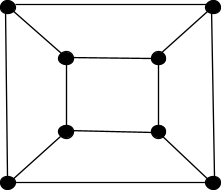
\includegraphics[width=.2\linewidth]{resources/3-regular graph.png}
\end{center}
\begin{itemize}
  \item A graph $H = (V_H,E_H)$ is a \bld{subgraph} of a graph $G = (V_G,E_G)$ if $V_H \subseteq V_G \tand E_H \subseteq E_G$. Note that any graph $G$ is a subgraph of itself.
\end{itemize}
\begin{center}
  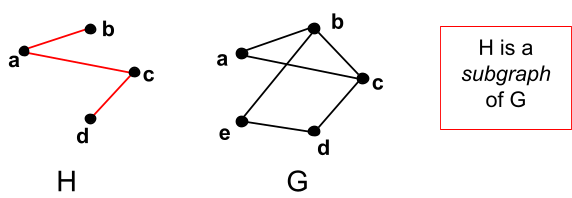
\includegraphics[width=.6\linewidth]{resources/H is a subgraph of G.png}
\end{center}

\subsubsection*{Theorem: Number of Edges and Total Degree}
Let $G = (V,E)$ be an undirected graph, simple or not. Then, twice the number of edges is equal to the total degree:
\[
  \sum_{v \in V} \deg(v) = 2 \cdot |E|
\]

\subsubsection*{Common Graphs}
Some graphs with special structure are given their own name and notation because they come up so frequently in graph theory.
\begin{center}
  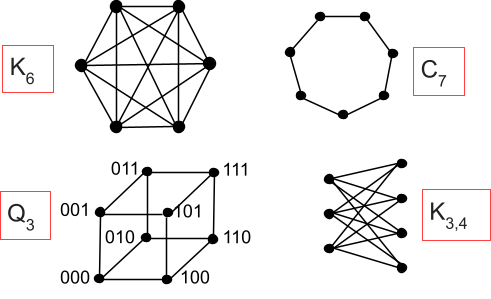
\includegraphics[width=0.7\linewidth]{resources/common graphs.png}
\end{center}
For the definition of all of these graphs, $n \in \bb{Z}^+$.
\begin{itemize}
  \item $K_n$ is called the \bld{complete graph} on $n$ vertices. $K_n$ has an edge between every pair of vertices. $K_n$ is sometimes called a \bld{clique} of size $n$ or an \bld{$n$-clique}.
  \item $C_n$ is called a cycle on $n$ vertices. The edges connect the vertices in a ring. Note that $C_n$ is well defined only for $n \geq 3$.
  \item The $n$-dimensional hypercube, denoted $Q_n$, has $2^n$ vertices. Each vertex is label with an $n$-bit string. Two vertices are connected by an edge if their corresponding labels differ only by one bit.
  \item $K_{n,m}$ has $n+m$ vertices, and $2nm$ edges. The vertices are divided into two sets: one with $m$ vertices and one set with $n$ vertices. There are no edges between vertices in the same set, but there is an edge between every vertex in one set and every vertex in the other set.
\end{itemize}

\subsection{Graph representations}
\begin{center}
  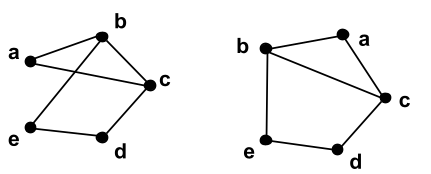
\includegraphics[width=0.5\linewidth]{resources/two similar graphs.png}
\end{center}
These two graphs look different, but that is only because they are drawn differently. The two graphs are actually the same graph because they have the same vertex and edge sets as shown below:
\begin{align*}
  V & = \{a,b,c,d,e\}                                       \\
  E & = \{\{a,b\},\{a,c\},\{b,c\},\{b,e\},\{c,d\},\{d,e\}\}
\end{align*}
The way a graph is drawn is not part of the graph itself.

\subsubsection*{Adjacency List Representation for Graphs}
In the \bld{adjacency list representation} of a graph, each vertex has a list of all its neighbors. Note that since the graph is undirected if vertex $a$ is in $b$'s list of neighbors, then $b$ must also be in $a$'s list of neighbors.

If a graph is represented using adjacency lists, the time required to list the neighbors of a vertex $v$ is proportional to $\deg(v)$, the number of vertices to be listed. In order to determine if $\{a,b\}$ is an edge, it is necessary to scan the list of $a$'s neighbors or the list of $b$'s neighbors. In the worst case, the time required is proportional to the larger of $\deg(a)$ or $\deg(b)$.

\subsubsection*{Matrix Representation for Graphs}
The \bld{matrix representation} for a graph with $n$ vertices is an $n \times n$ matrix whose entries are all either $0 \tor 1$, indicating whether or not each edge is present. The matrix representation of an undirected graph is symmetric.
\begin{center}
  \begin{tikzpicture}
    %VARIABLES
    \pgfmathsetmacro{\gsize}{1};
    \pgfmathsetmacro{\gnum}{5};

    \foreach[count=\i] \element in {a,b,c,d,e} { %domain
        \node (\element) at (\i * 360 / \gnum:\gsize) {$\element$};
        \node (\element-) at (\i * 360 / \gnum:\gsize + 0.5) {};
      }
    \foreach \j/\l in {a/b,a/c,b/c,b/e,c/d,d/e} { %a to b
        \draw (\j) -- (\l);
      }
    \node[anchor=east] (name) at (145:\gsize+.5) {}; %relation name
  \end{tikzpicture} $~~\Rightarrow~~$
  $
    \begin{bmatrix}
      0 & 1 & 1 & 0 & 0 \\
      1 & 0 & 1 & 0 & 1 \\
      1 & 1 & 0 & 1 & 0 \\
      0 & 0 & 1 & 0 & 1 \\
      0 & 1 & 0 & 1 & 0
    \end{bmatrix}
  $
\end{center}

\subsection{Graph isomorphism}
Two graphs are said to be \bld{isomorphic} if there is a correspondence between the vertex sets of each graph such that there is an edge between two vertices of one graph if and only if there is an edge between the corresponding vertices of the second graph. Essentially, the graphs are not identical but the vertices can be relabeled so that they are identical.

\subsubsection*{Definition of Isomorphic Graphs}
Let $G = (V,E) \tand G'=(V',E')$. $G \tand G'$ are isomorphic if there is a bijection $f: V \rightarrow V'$ such that for every pair of vertices $x,y \in V$, $\{x,y\} \in E$ if and only if $\{f(x), f(y)\} \in E'$. The function $f$ is called an \bld{isomorphism} from $G \tto G'$.

\begin{center}
  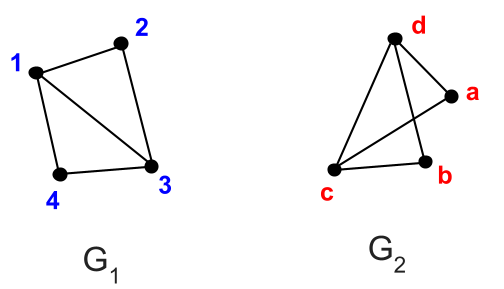
\includegraphics[width=0.5\linewidth]{resources/isomorphic graphs 1.png}
\end{center}
The following function is an isomorphism from the vertices of $G_1 \tto G_2$:
\[
  f(1) = d \qquad f(2) = a \qquad f(3) = c \qquad f(4) = b
\]

\subsubsection*{Theorem: Vertex Degree Preserved under Isomorphism}
Consider two graphs, $G \tand G'$. Let $f$ be an isomorphism from $G \tto G'$. For each vertex $v \tin G$, the degree of vertex $v \tin G$ is equal to the degree of vertex $f(v) \tin G'$.

\subsubsection*{}
The \bld{degree sequence} of a graph is a list of the degree of all of the vertices in non-increasing order.
\begin{center}
  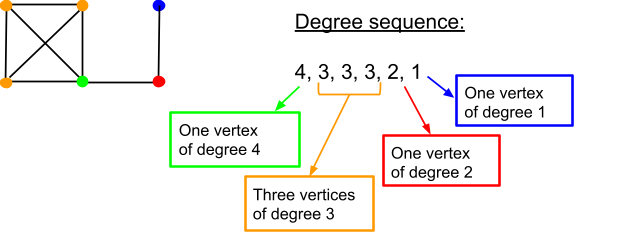
\includegraphics[width=0.7\linewidth]{resources/degree-sequence.png}
\end{center}

\subsubsection*{Theorem: Degree Sequence Preserved under Isomorphism}
The degree sequence of a graph is preserved under isomorphism.


\subsection{Walks, trails, circuits, paths, and cycles}
A \bld{walk} from $v_0 \tto v_l$ in an undirected graph $G$ is a sequence of alternating vertices and edges that starts and ends with a vertex:
\[
  \langle v_0,\{v_0,v_1\},v_1,\{v_1,v_2\},\ldots,v_{\ell-1},\{v_{\ell-1},v_\ell\},v_\ell\rangle
\]
Since the edges in a walk are completely determined by the vertices, a walk can also be denoted by the sequence of vertices:
\[
  \langle v_0,v_1,\ldots,v_\ell \rangle.
\]
However, keep in mind the sequence of vertices is a walk only if $\{v_{j-1},v_j\} \in E$ for each $j = 1,2,\ldots,\ell$. The \bld{length of a walk} is $\ell$, the number of edges in the walk. An \bld{open walk} is a walk in which the first and last vertices are not the same. A \bld{closed walk} is a walk in which the first and last vertices are the same.
\begin{itemize}
  \item A \bld{trail} is a walk in which no \itl{edge} occurs more than once.
  \item A \bld{path} is a walk in which no \itl{vertex} occurs more than once.
  \item A \bld{circuit} is a closed \itl{trail}.
  \item A \bld{cycle} is a \itl{circuit} is length at least 1 in which no vertex occurs more than once, except the first and last vertices which are the same.
\end{itemize}
Here are some examples of closed walks:
\begin{itemize}
  \item $\langle A,C,D,A \rangle$ is a \itl{trail}, a \itl{circuit}, and a \itl{cycle}.
  \item $\langle A,C,B,A,D,E,A \rangle$ is a \itl{trail} and a \itl{circuit}.
  \item $\langle A,B,A \rangle$ is \bld{not} a trail, circuit, or a cycle.
\end{itemize}
Since paths and cycles do not have any repeated edges, if a graph is simple, any cycle \itl{must} have length at least 3. The sequence $\langle v \rangle$ is not a cycle because a cycle, by definition, must have length at least 1. The sequence $\langle v,v \rangle$ is only a walk if there is a self-loop at vertex $v$.

\subsection{Graph connectivity}
Two vertices, $v \tand w$, are \bld{connected} if there is a path from $v \tto w$ (and thus also a path from $w \tto v$). A vertex is always considered to be connected to itself. The property of being connected can be extended to sets of vertices and the entire graph:
\begin{itemize}
  \item A set of vertices in a graph is said to be connected if every pair of vertices in the set is connected.
  \item A graph is said to be connected if every pair of vertices in the graph is connected, and is \bld{disconnected} otherwise.
\end{itemize}
A \bld{connected component} consists of a \itl{maximal} set of vertices that are connected as well as all the edges between two vertices in the set. A vertex that is not connected with any other vertex is called an \bld{isolated vertex} and is therefore a connected component with only one vertex.
\begin{center}
  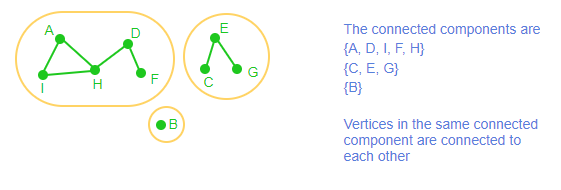
\includegraphics[width=0.6\linewidth]{resources/connected components example.png}
\end{center}

\subsubsection*{k-Connectivity}
In some networks, it is important to be able to guarantee connectivity, even if one or more vertices or edges are removed from a graph. The definition of connectivity can be extended to encompass resilience to vertex or edge failures.

\subsubsection*{Definition of a K-vertex-connected Graph}
An undirected graph $G$ is \bld{$k$-vertex-connected} if the graph contains at least $k + 1$ vertices and remains connected after any $k - 1$ vertices are removed from the graph. The \bld{vertex connectivity} of a graph is the largest $k$ such that the graph is $k$-vertex-connected. The vertex connectivity of a graph $G$ is denoted $\kappa(G)$.

The vertex connectivity of a graph is the minimum number of vertices whose removal disconnects the graph into more than one connected component.

When the graph is a complete graph, there is no set of vertices whose removal disconnects the graph. For the special case of $K_n$, the vertex connectivity $\kappa(K_n)$ is just defined to be $n - 1$.

\subsubsection*{Definition of a K-edge-connected Graph}
An undirected graph G is \bld{$k$-edge-connected} if removing any $k - 1$ or fewer edges results in a connected graph. The \bld{edge connectivity} of a graph is the largest $k$ such that the graph is $k$-edge-connected. The edge connectivity of a graph G is denoted $\lambda(G)$.

The edge connectivity of a graph is the minimum number of edges whose removal disconnects the graph into more than one connected component.

\subsubsection*{Theorem: Upper bound for Vertex and Edge Connectivity}
Let $G$ be an undirected graph. Denote the minimum degree of any vertex in $G$ by $\delta(G)$. Then,
\begin{align*}
  \kappa(G)  & \leq \delta(G)~~~\tand \\
  \lambda(G) & \leq \delta(G).
\end{align*}

\subsection{Euler circuits and trails}
An \bld{Euler circuit} is a circuit that contains every edge and every vertex. Note that a circuit, by definition, has no repeated edges, so an Euler circuit contains each edge exactly once.
\begin{center}
  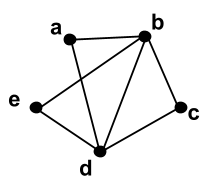
\includegraphics[width=0.25\linewidth]{resources/euler circuit example.png}
  Euler circuit: $\langle a,b,c,d,e,b,d,a \rangle$
\end{center}

\subsubsection*{Theorem: Characterization of Graphs that have an Euler Circuit}
An undirected graph $G$ has an Euler circuit if and only if $G$ is connected and every vertex in $G$ has even degree.
\[
  G~\text{has an Euler circuit}~\leftrightarrow G~\text{is connected and every vertex in $G$ has even degree}.
\]

\subsubsection*{Procedure to find a circuit in a Graph}
\begin{lstlisting}
Find a vertex w, that is not an isolated vertex.
Select any edge {w,x} incident to w.
(Since w is not isolated, there is always at least one such edge.)
Current trail T := <w,x>
last := x
While there is an edge {last, y} that has not been used in T:
  Add y to the end of T
  last := y
\end{lstlisting}

\subsubsection*{Procedure to find an Euler circuit in a Graph}
Use the procedure above to find any circuit in $G$. Call the circuit $C$. The algorithm continues to iterate the following steps until all the edges in $G$ are included in $C$:
\begin{enumerate}
  \item Remove all edges in $C$ from $G$. Remove any isolated vertices from $G$. Call the resulting graph $G'$.
  \item Find a vertex $w$ that is in $G' \tand C$.
  \item Find a circuit in $G'$ that begins and ends with $w$. Call the circuit $C'$.
  \item Combine circuit $C \tand C'$. Suppose $C$ starts and ends at vertex $v$. Create a new circuit that starts at $v$ and follows the edges in $C$ until $w$ is reached. The new circuit then follows the edges in $C'$ back to $w$ and then follows the rest of the edges in $C$ back to $v$. The new circuit is renamed $C$ for the next iteration.
\end{enumerate}


\subsubsection*{Euler trail}
An \bld{Euler trail} is an open trail that includes each edge. Note that a trail, by definition, has no repeated edges, so an Euler trail contains each edge exactly once. In an open trail, the first and last vertices are not equal.

\subsubsection*{Theorem: Characterizations of graphs that have an Euler trail}
An undirected graph $G$ has an Euler trail if and only if $G$ is connected and has exactly two vertices with odd degree. The Euler trail begins and ends with the vertices of odd degree.
\[
  G~\text{has an Euler trail}~\leftrightarrow G~\text{is connected and has exactly two vertices with odd degree}.
\]

\subsection{Hamiltonian cycles and paths}
A \bld{Hamiltonian cycle} in an undirected graph is a cycle that includes every vertex in the graph. Note that a cycle, by definition, has no repeated vertices or edges, except for the vertex which is at the beginning and end of the cycle. Therefore, every vertex in the graph appears exactly once in a Hamiltonian cycle, except for the vertex which is at the beginning and end of the cycle. A \bld{Hamiltonian path} in an undirected graph is a path that includes every vertex in the graph. Note that a path, by definition, has no repeated vertices or edges, so every vertex appears exactly once in a Hamiltonian path.

Note that a Hamiltonian cycle can be transformed into a Hamiltonian path by deleting the last vertex. Therefore if a graph has a Hamiltonian cycle, then the graph also has a Hamiltonian path.

Unlike Euler circuits and trails, there are no known conditions describing exactly which graphs have a Hamiltonian cycle or path. However, there are some cases in which a graph that does have a Hamiltonian cycle or path has a certain property.
\begin{itemize}
  \item Any graph that has a vertex with degree 1 does not have a Hamiltonian cycle.
  \item For $n \geq 3$, $K_n$ has a Hamiltonian cycle.
\end{itemize}

\subsection{Planar graphs}
Placing graphs on two-dimensional surfaces to avoid crossings is a classic problem in graph theory. The problem also arises in the field of graph drawing in which the goal is to draw complex graphs in a way that helps people visualize structure and patterns.

An \bld{embedding} for $G = (V,E)$ is an assignment of the vertices to points in the plane and an assignment of each edge to a continuous curve. The curve for each edge must start and edge at the two points corresponding to the endpoints of the edge. Essentially, an \itl{embedding is a way of drawing a graph} on a plane, because mathematically, a graph is just a set of vertices and a set of edges.

An embedding is said to be a \bld{planar embedding} if none of the edges cross. There is a crossing between two edges in an embedding if their curves intersect at a point that is not a common endpoint. An embedding of a graph can be planar or not planar, depending on whether it has a crossing. Planarity can also be defined as a property of the graph itself.

\subsubsection*{Definition of Planar Graphs}
A graph $G$ is a \bld{planar graph} if the graph has a planar embedding.

\begin{center}
  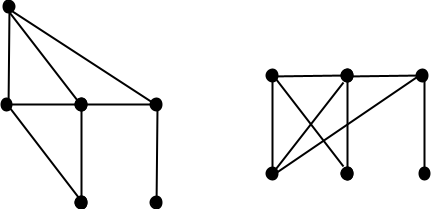
\includegraphics[width=0.4\linewidth]{resources/two embeddings.png}
\end{center}
\begin{itemize}
  \item The embedding on the left \itl{is planar}.
  \item The embedding on the right \itl{is \bld{not} planar}.
\end{itemize}

The \bld{complement of an embedding} is the set of all points in the plane that are not part of a curve corresponding to an edge. A planar embedding carves up the plane into continuous regions. A \bld{region} is a set of points in the complement of an embedding that forms a maximal continuous set, meaning that it is (continuous): possible to travel anywhere from any point in the region and (maximal): if any point were added to the region, it would no longer be continuous. In a planar embedding, there is always an infinite region called the \bld{exterior region}, which is region $V$ in the following graph.
\begin{center}
  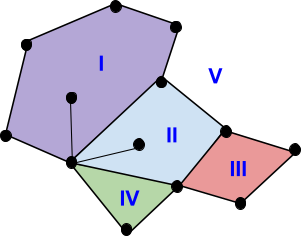
\includegraphics[width=0.4\linewidth]{resources/regions of a planar embedding.png}
\end{center}

\subsubsection*{Theorem: Euler's Identity for Regions in an Embedding}
Consider a planar embedding of a connected graph $G$. Let $v$ be the number of vertices in $G$, $e$ the number of edges, and $r$ the number of regions in the embedding. Then,
\[
  v - e + r = 2
\]

\subsubsection*{Degree of a Region}
\begin{center}
  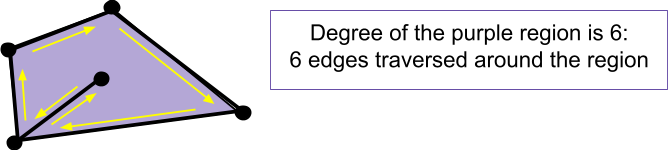
\includegraphics[width=0.7\linewidth]{resources/degree of a region.png}
\end{center}
Consider a planar embedding of a graph G. Think of a tiny bug walking all the way around the region along the edges of the graph. The degree of a region is the number of times the bug traverses an edge until it gets back to its starting location. Note that if an edge sticks out into a region, the edge can be traversed twice by the bug and therefore contributes 2 towards the degree of the region.

\subsubsection*{Theorem: Number of Edges in a Planar Graph}
Let G be a connected planar graph. Let $v$ be the number of vertices in G and $e$ the number of edges. If $v \geq 3$, then
\[
  e \leq 3v-6
\]

\subsection{Graph coloring}

\section{Trees}
\subsection{Introduction to trees}
\begin{center}
  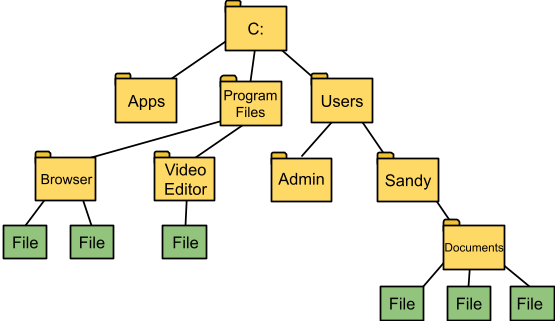
\includegraphics[width=0.6\linewidth]{resources/diagram of a file system.png}
\end{center}
The file system can be seen as a graph in which each folder or file is a vertex. There is an edge between two folders if one folder is a subfolder of the other. There is an edge between a file and a folder if the file resides in that folder. In most computer operating systems, a file or folder can only reside in one location, which means that the underlying graph corresponds to a tree.

\subsubsection*{Definition of a Tree}
A \bld{tree} is an undirected graph that is connected and has no cycles.

\subsubsection*{Free Trees and Rooted Trees}
\begin{center}
  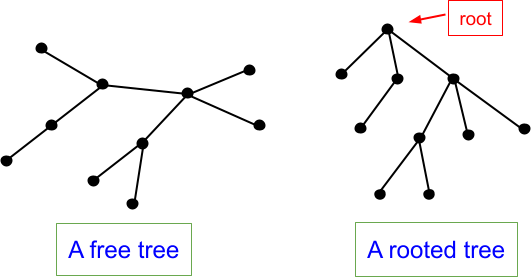
\includegraphics[width=0.5\linewidth]{resources/free and rooted trees.png}
\end{center}
The tree on the left is called a \bld{free tree} because there is no particular organization of the vertices and edges. The tree on the right is called a \bld{rooted tree}. The vertex at the top of the drawing is designated as the \bld{root} of the tree. The remaining vertices are organized according to their distance from the root. The distance between two vertices in an undirected graph is the number of edges in the shortest path between the two vertices. The \bld{level} of a vertex is its distance from the root. The \bld{height} of a tree is the highest level of any vertex. The tree on the right has height 3.

\subsubsection*{Theorem: Unique Paths in Trees}
Let $T$ be a tree and let $u \tand v$ be two vertices in $T$. There is \itl{exactly one path} between $u \tand v$.

\subsubsection*{Terminology related to Rooted Trees}
\begin{itemize}
  \item Every vertex in a rooted tree $T$ has a unique \bld{parent}, except for the root which does not have a parent. The parent of vertex $v$ is the first vertex encountered along the path from $v$ to the root.
  \item Every vertex along the path from $v$ to the root, except for the vertex $v$ itself, is an \bld{ancestor} of vertex $v$.
  \item If $v$ is the parent of vertex $u$, then $u$ is a \bld{child} of vertex $v$.
  \item If $u$ is an ancestor of $v$, then $v$ is a \bld{descendant} of $u$.
  \item A \bld{leaf} is a vertex which has no children.
  \item Two vertices are \bld{siblings} if they have the same parent.
  \item A \bld{subtree} rooted as vertex $v$ is the tree consisting of $v$ and all of $v$'s descendants.
\end{itemize}

\subsubsection*{Forests}
A \bld{forest} is a graph that has no cycles but is not necessarily connected. The picture below shows a forest with 3 connected components.
\begin{center}
  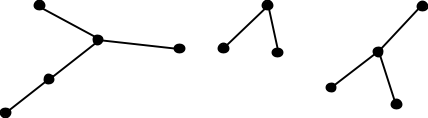
\includegraphics[width=0.6\linewidth]{resources/forest example.png}
\end{center}

\subsection{Tree application examples}

\subsubsection*{Game Trees}
\begin{center}
  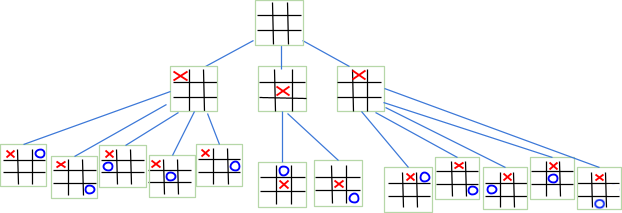
\includegraphics[width=0.7\linewidth]{resources/tictactoe game tree.png}
\end{center}
The root of the tree is the initial configuration of the game. In the case of tic-tac-toe, the initial configuration is an empty grid. The odd levels of the game tree represent choices of play for the X player and the even levels represent choices of play for the O player. The children of a configuration c are all the configurations that can be reached from c by a single move of the correct player. A configuration is a leaf vertex in the tree if the game is over.

Theoretically, a game tree can be systematically analyzed to determine optimal playing strategies for each player. However, in practice for most games, the corresponding game tree is much too large to build and analyze in its entirety. Programs like Deep Blue build partial game trees starting from the current configuration in the game and estimate the best next move based on the results of the partial tree.

Tic-tac-toe and chess are examples of deterministic games whose outcome is completely determined by the choices made by each player. A game that involves rolling a pair of dice or shuffling a deck of cards introduces randomization into the game. Probability theory as well as game trees are required to analyze games with an element of chance.

\subsubsection*{Prefix Codes}
Space-efficient encodings can be achieved by \bld{variable length codes}, in which the number of bits for each character can vary. Characters such as "a" and "e" that occur frequently are represented with fewer bits, while characters such as "z" or "q" are represented using more bits.

Trees are a convenient way to represent variable length codes for translating between text and binary.
\begin{center}
  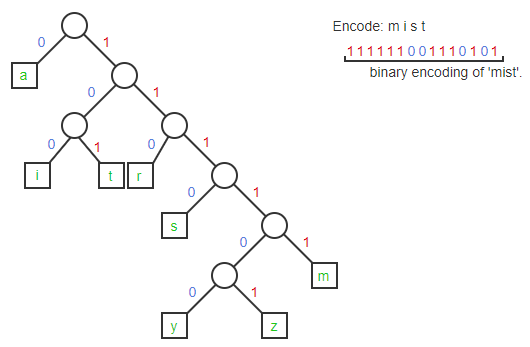
\includegraphics[width=0.6\linewidth]{resources/variable length encoding example.png}
\end{center}
The code illustrated in the animation is an example of a prefix code. A string $s$ is a \bld{prefix} of another string $t$ if all the characters in string $s$ appear at the beginning of string $t$.
\begin{center}
  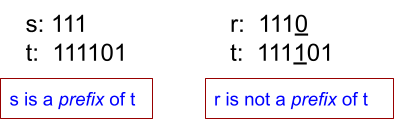
\includegraphics[width=0.4\linewidth]{resources/string prefix example.png}
\end{center}
A \bld{prefix code} has the property that the code for one character \itl{can not} be a prefix of the code for another character. The fact that the codes are organized as a tree in which characters are only stored at the leaves ensures the prefix property.

\subsection{Properties of trees}

\subsubsection*{Theorem: Unique Paths in Trees}
There is a unique path between every pair of vertices in a tree.

\subsubsection*{Theorem: Number of Leaves in a Tree}
Any free tree with at least two vertices has at least two leaves.

\subsubsection*{Theorem: Number of Edges in a Tree}
Let $T$ be a tree with $v$ vertices and $e$ edges. Then
\[
  e = v-1.
\]

\subsection{Tree traversals}
A common procedure performed on a tree, called a \bld{tree traversal}, is to process the information stored in the vertices by systematically visiting each vertex. In a \bld{pre-order traversal}, a vertex is visited before its descendants. In a \bld{post-order traversal}, a vertex is visited after its descendants.

\subsubsection*{Pseudocode and Example for Pre-order Traversal}
\begin{lstlisting}
Pre-order(v)

process(v) // process happens first
For every child w of v:
  Pre-order(w)
End-for
\end{lstlisting}
\begin{center}
  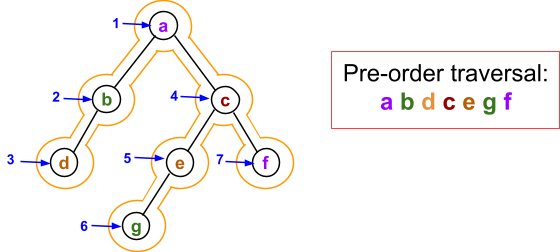
\includegraphics[width=0.4\linewidth]{resources/preorder traversal.png}
\end{center}

\subsubsection*{Pseudocode and Example for Post-order Traversal}
\begin{lstlisting}
Post-order(v)

For every child w of v:
  Post-order(w)
End-for
process(v) // process happens last
\end{lstlisting}
\begin{center}
  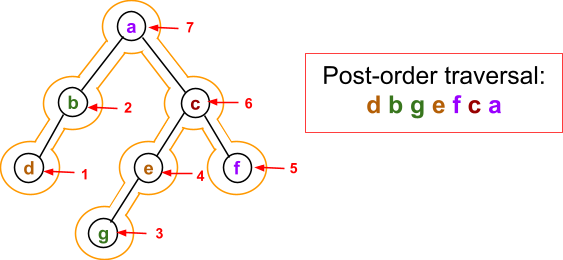
\includegraphics[width=0.4\linewidth]{resources/post order traversal.png}
\end{center}

\subsection{Spanning trees and graph traversals}
Suppose an application needs to broadcast information to every computer (vertex) in a network. The information will be disseminated along the communication links so that every vertex in the network receives the information. Moreover, the goal is to minimize overall congestion, so it would be wasteful to send information along alternate paths to the same location. The information should be broadcast over a spanning tree of the network. Here is the formal definition of a spanning tree:

\subsubsection*{Definition of a Spanning Tree of a Connected Graph}
A \bld{spanning tree} of a connected graph $G$ is a subgraph of $G$ which contains all the vertices in $G$ and is a tree.

\subsubsection*{}
The picture below shows several possible spanning trees of the same graph. The edges of the spanning tree are shown in red. The vertex set of the spanning tree is always the entire set of vertices in the graph.
\begin{center}
  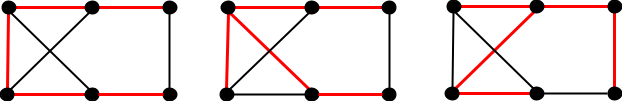
\includegraphics[width=0.6\linewidth]{resources/spanning trees example.png}
\end{center}

\subsubsection*{Graph Traversals}
There are two common methods for finding spanning trees in a graph: Breadth-First Search and Depth-First Search. Both methods start at a single vertex and incrementally build a connected tree by adding edges and vertices. The resulting tree is rooted at the start vertex. Graph traversal is a process that systematically explores all the vertices of a graph.

\subsubsection*{Depth-First Search}
As the name suggests, Depth-First Search (DFS) favors going deep into the graph and tends to produce trees with longer paths from the start vertex.
\begin{lstlisting}
Depth-first-search

Input: An undirected, connected graph G. A start vertex v[1]
Output: T, a depth-first search tree.

Add v[1] to T.
visit(v[1])

visit(v)

For every neighbor w of v:
  If w is not already in T
    Add w and {w, v} to T.
    visit(w);
  End-if
End-for
\end{lstlisting}
Note that there is some ambiguity with regard to the order in which the neighbors of a vertex are considered.

\subsubsection*{Breath-first Search}
Breadth-First Search (BFS) explores the graph by distance from the initial vertex, starting with its neighbors and expanding the tree to neighbors of neighbors, etc. Breadth-first-search visits vertices in the graph according to their proximity to the start vertex. The algorithm maintains a list of vertices to be visited soon. Vertices are added to the back of the list and the next vertex to visit is taken from the front of the list.
\begin{lstlisting}
Breadth-first-search

Input: An undirected, connected graph G. A start vertex v[1]
Output: T, a breadth-first search tree.

Add v[1] to T.
Add v[1] to the back of the list.

While the list is not empty:
  Remove vertex v from the front of the list.
  For each neighbor w of v that is not already in T:
    Add w and {w, v} to T.
    Insert w at the back of the list.
  End-for
End-while
\end{lstlisting}

\subsection{Minimum spanning trees}
When edges have varying costs, a natural goal is to minimize the total cost of the spanning tree.

\subsubsection*{Definition of a Weighted Graph}
A \bld{weighted graph} is a graph $G = (V,E)$, along with a function $w: E \rightarrow \bb{R}$. The function $w$ assigns a real number to each edge.
\begin{center}
  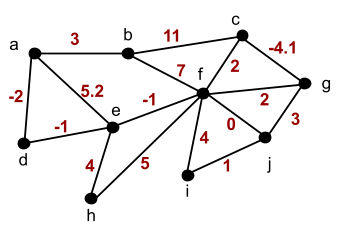
\includegraphics[width=0.6\linewidth]{resources/example weighted graph.png}
\end{center}
When the goal is to span the vertices of the graph while minimizing the total weight of the edges used, a \bld{minimum spanning tree} can be used.

\subsubsection*{Definition of a Minimum Spanning Tree}
A \bld{minimum spanning tree} (MST) of a weighted graph is a spanning tree $T$ of $G$ whose weight is no larger than any other spanning tree of $G$.

\subsubsection*{Prim's Algorithm for Minimum Spanning Trees}
This is a classic algorithm for finding minimum spanning trees, developed by mathematician Robert Prim in 1957.
\begin{lstlisting}
Input: An undirected, connected, weighted graph G.
Output: T, a minimum spanning tree for G.

T := {}.
Pick any vertex in G and add it to T.

For j = 1 to n-1
  Let C be the set of edges with one endpoint inside T 
      and one endpoint outside T.
  Let e be a minimum weight edge in C.
  Add e to T.
  Add the endpoint of e not already in T to T.
End-for
\end{lstlisting}

\subsubsection*{Theorem: Result of Prim's Algorithm}
Prim's algorithm finds a minimum spanning tree of the input weighted graph.

\end{document}